\section{Efficiency determination}
\label{Efficiency determination}
The number of signal candidates are corrected by the total efficiency to obtain the \psitwos-to-\jpsi cross-section ratio measurements. The efficiencies are assumed to be equal for prompt and from-$b$ signals as can be seen for example in the measurement of \jpsi cross-section at 13 TeV. The total efficiency is the product of the acceptance efficiency (\effAcc), the reconstruction and selection efficiency (\effReco), the particle identification efficiency (\effID), the trigger efficiency (\effTrigger). The acceptance efficiency is calculated for all multiplicity classes. The others are calculated in each multiplicity class. And according to Eq.~\ref{CS_ratio}, we are going to find the efficiency ratio in each multiplicity class. The ratio of total efficiencies for \jpsi and \psitwos is defined in the following equation~\ref{EffRatio}.
\begin{equation}
\begin{split}
R_{tot}=&\frac{\ensuremath{\epsilon_{\mathrm{tot,\jpsi}}}}{\ensuremath{\epsilon_{\mathrm{tot,\psitwos}}}}\bigg|_{Mult. \ bin} \\
= &\frac{\ensuremath{\epsilon_{\mathrm{acc,\jpsi}}}}{\ensuremath{\epsilon_{\mathrm{acc,\psitwos}}}}\times \frac{\ensuremath{\epsilon_{\mathrm{Reco\&Sel,\jpsi}}}\cdot\ensuremath{\epsilon_{\mathrm{MuonID,\jpsi}}}\cdot\ensuremath{\epsilon_{\mathrm{Trigger,\jpsi}}}}{\ensuremath{\epsilon_{\mathrm{Reco\&Sel,\psitwos}}}\cdot\ensuremath{\epsilon_{\mathrm{MuonID,\psitwos}}}\cdot\ensuremath{\epsilon_{\mathrm{Trigger,\psitwos}}}}\bigg|_{Mult. \ bin} \\
= &R_{acc}\times R_{eff}|_{Mult. \ bin},
\end{split}
\label{EffRatio}
\end{equation}
where $R_{acc}$ is the ratio of acceptance efficiencies of \jpsi to \psitwos and $R_{eff}$ is the ratio of the rest efficiencies of \jpsi and \psitwos. 
All steps are determined from simulation, with truth matched signal decays, except for the tracking efficiency and the particle identification, where data driven methods are used to correct the efficiencies obtained from the simulation. Their exact definitions are given in the following subsections. In the simulation, \jpsi and \psitwos mesons are assumed produced without polarization. For the simulation samples used for this analysis, the truth matching efficiency is equal to $99.5 \pm 0.1\%$ for both $p$Pb and Pb$p$ samples. It is assumed to be independent of \pt and $y^*$.

\subsection{Re-weight on Monte Carlo sample}
The distribution of $N_{\rm tracks}^{\rm PV}$, $N_{\rm fwd}^{\rm PV}$ and $N_{\rm bwd}^{\rm PV}$ of Monte Carlo and s-weight data for both \jpsi and \psitwos in $p$Pb and Pb$p$ configurations are compared. As an example, we draw the distributions for Monte Carlo and s-weight data in $p$Pb configuration in Figure~\ref{MulReweight}. We can see that the multiplicity distribution for \jpsi and \psitwos signals both in Monte Carlo sample and s-weight data are compatible within uncertainties. And what we want in the end is the ratio of total efficiencies. The bias caused by the difference in multiplicity should be canceled.
\begin{figure}[H]
\begin{center}
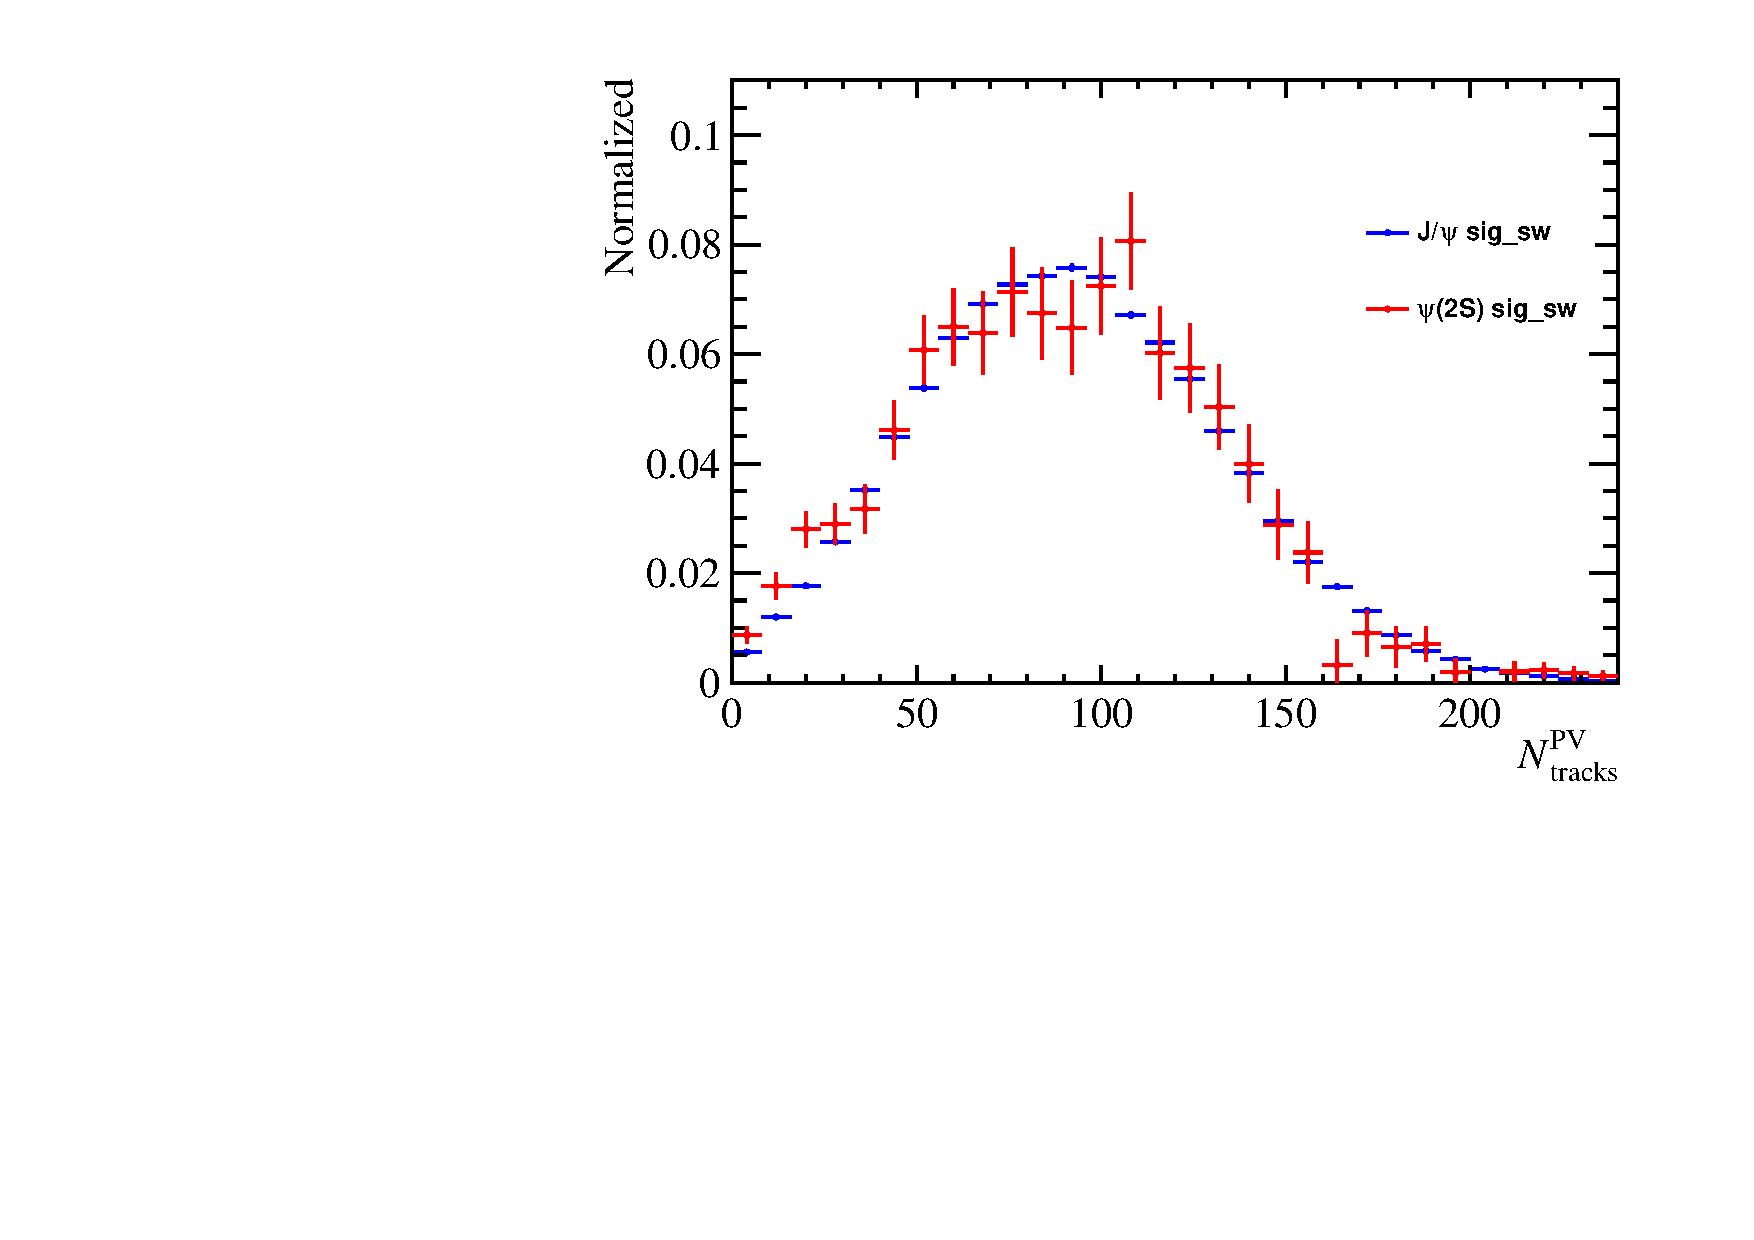
\includegraphics[width=0.32\linewidth]{pdf/pPb/Workdir/Reweight/sWeightMul.pdf}
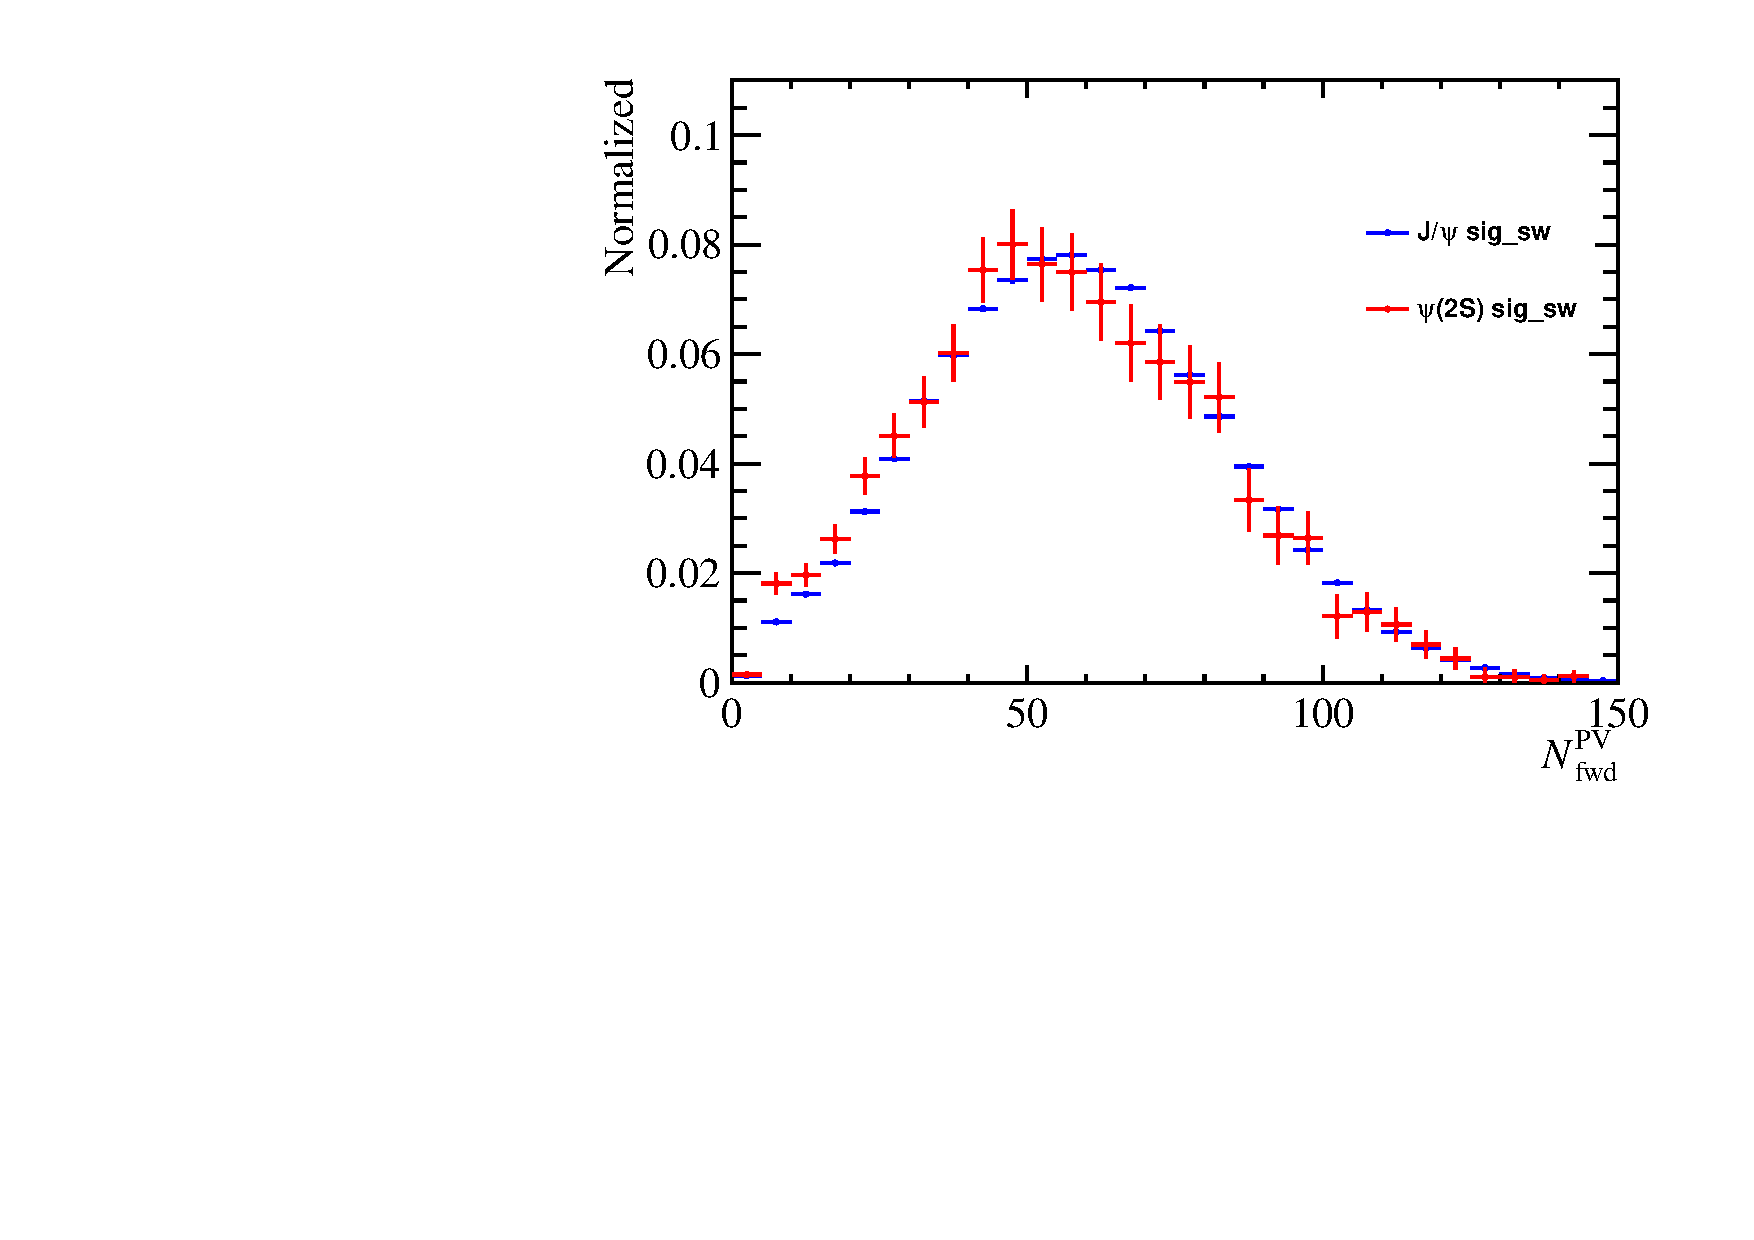
\includegraphics[width=0.32\linewidth]{pdf/pPb/FWorkdir/Reweight/sWeightMul.pdf}
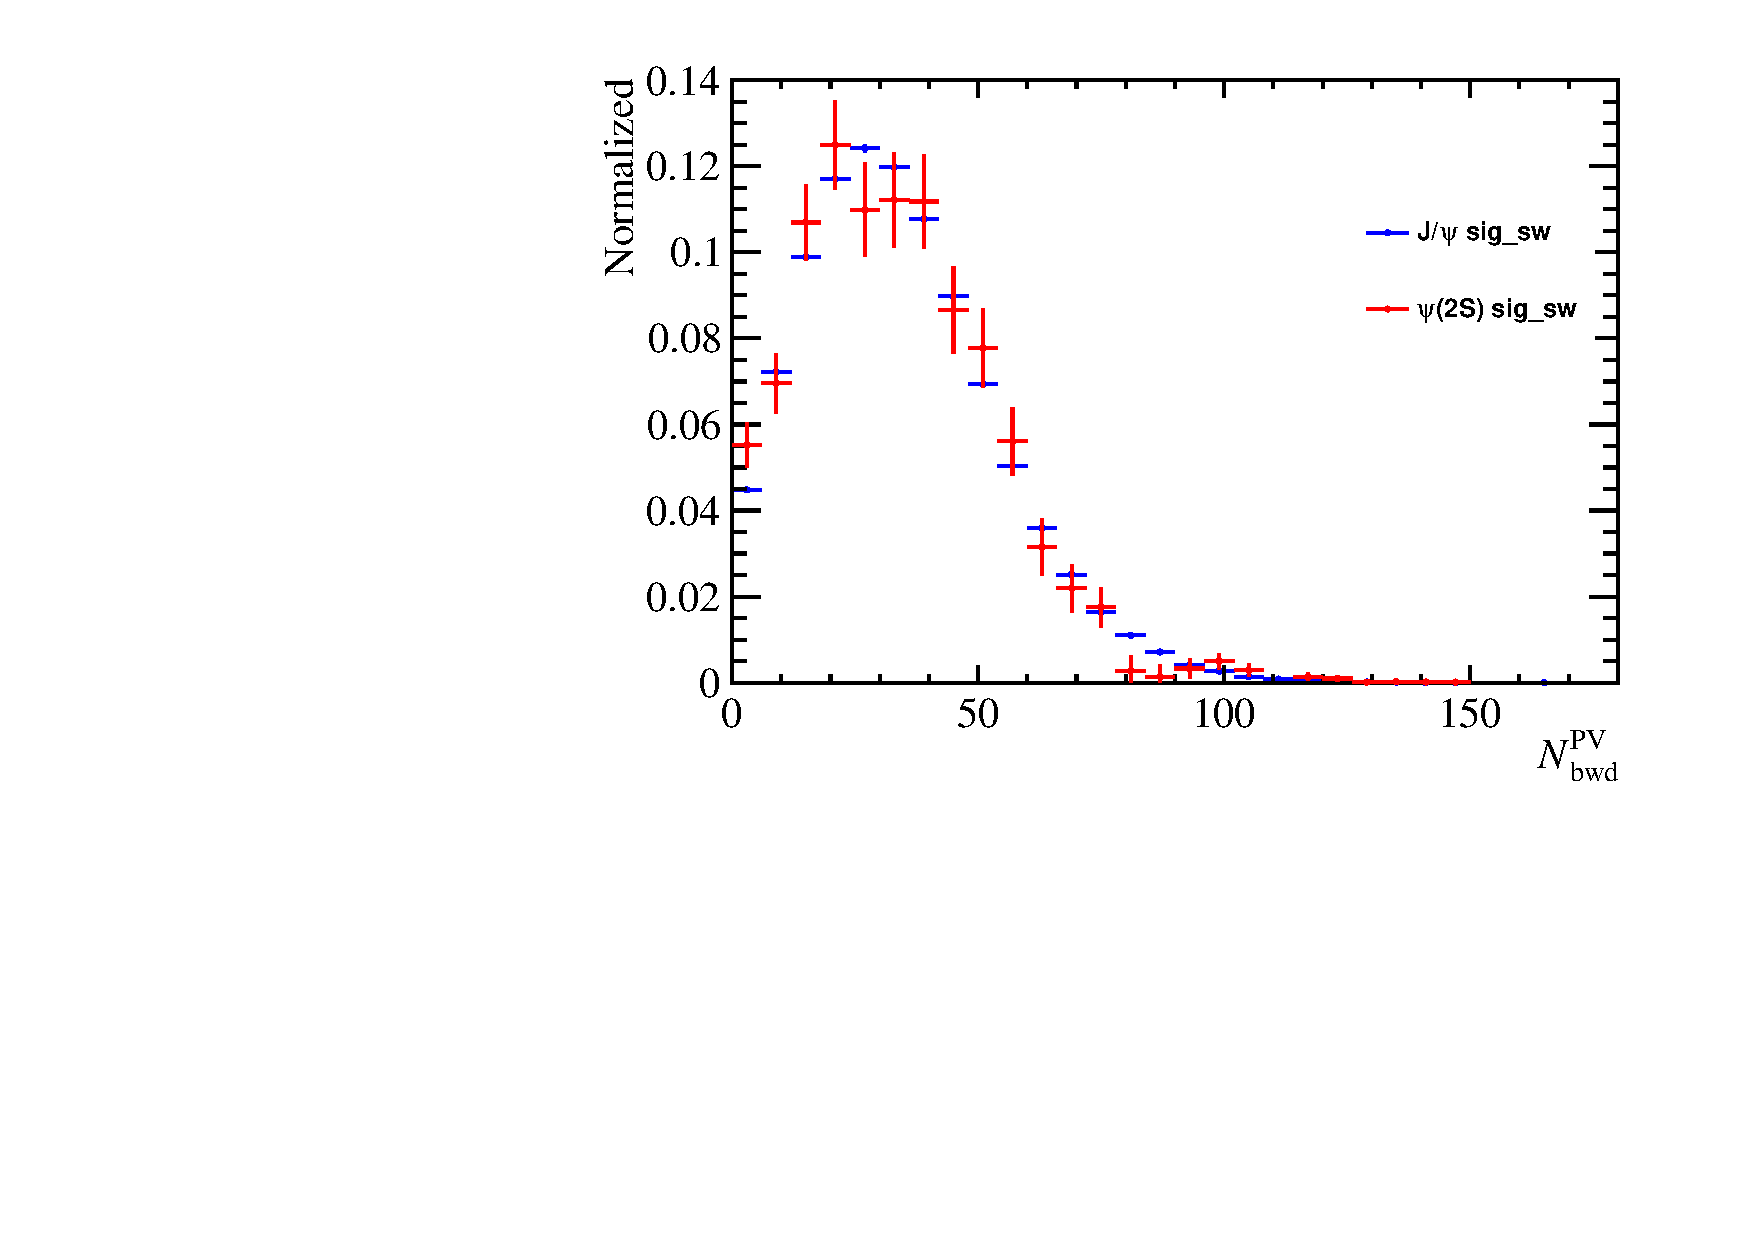
\includegraphics[width=0.32\linewidth]{pdf/pPb/BWorkdir/Reweight/sWeightMul.pdf}
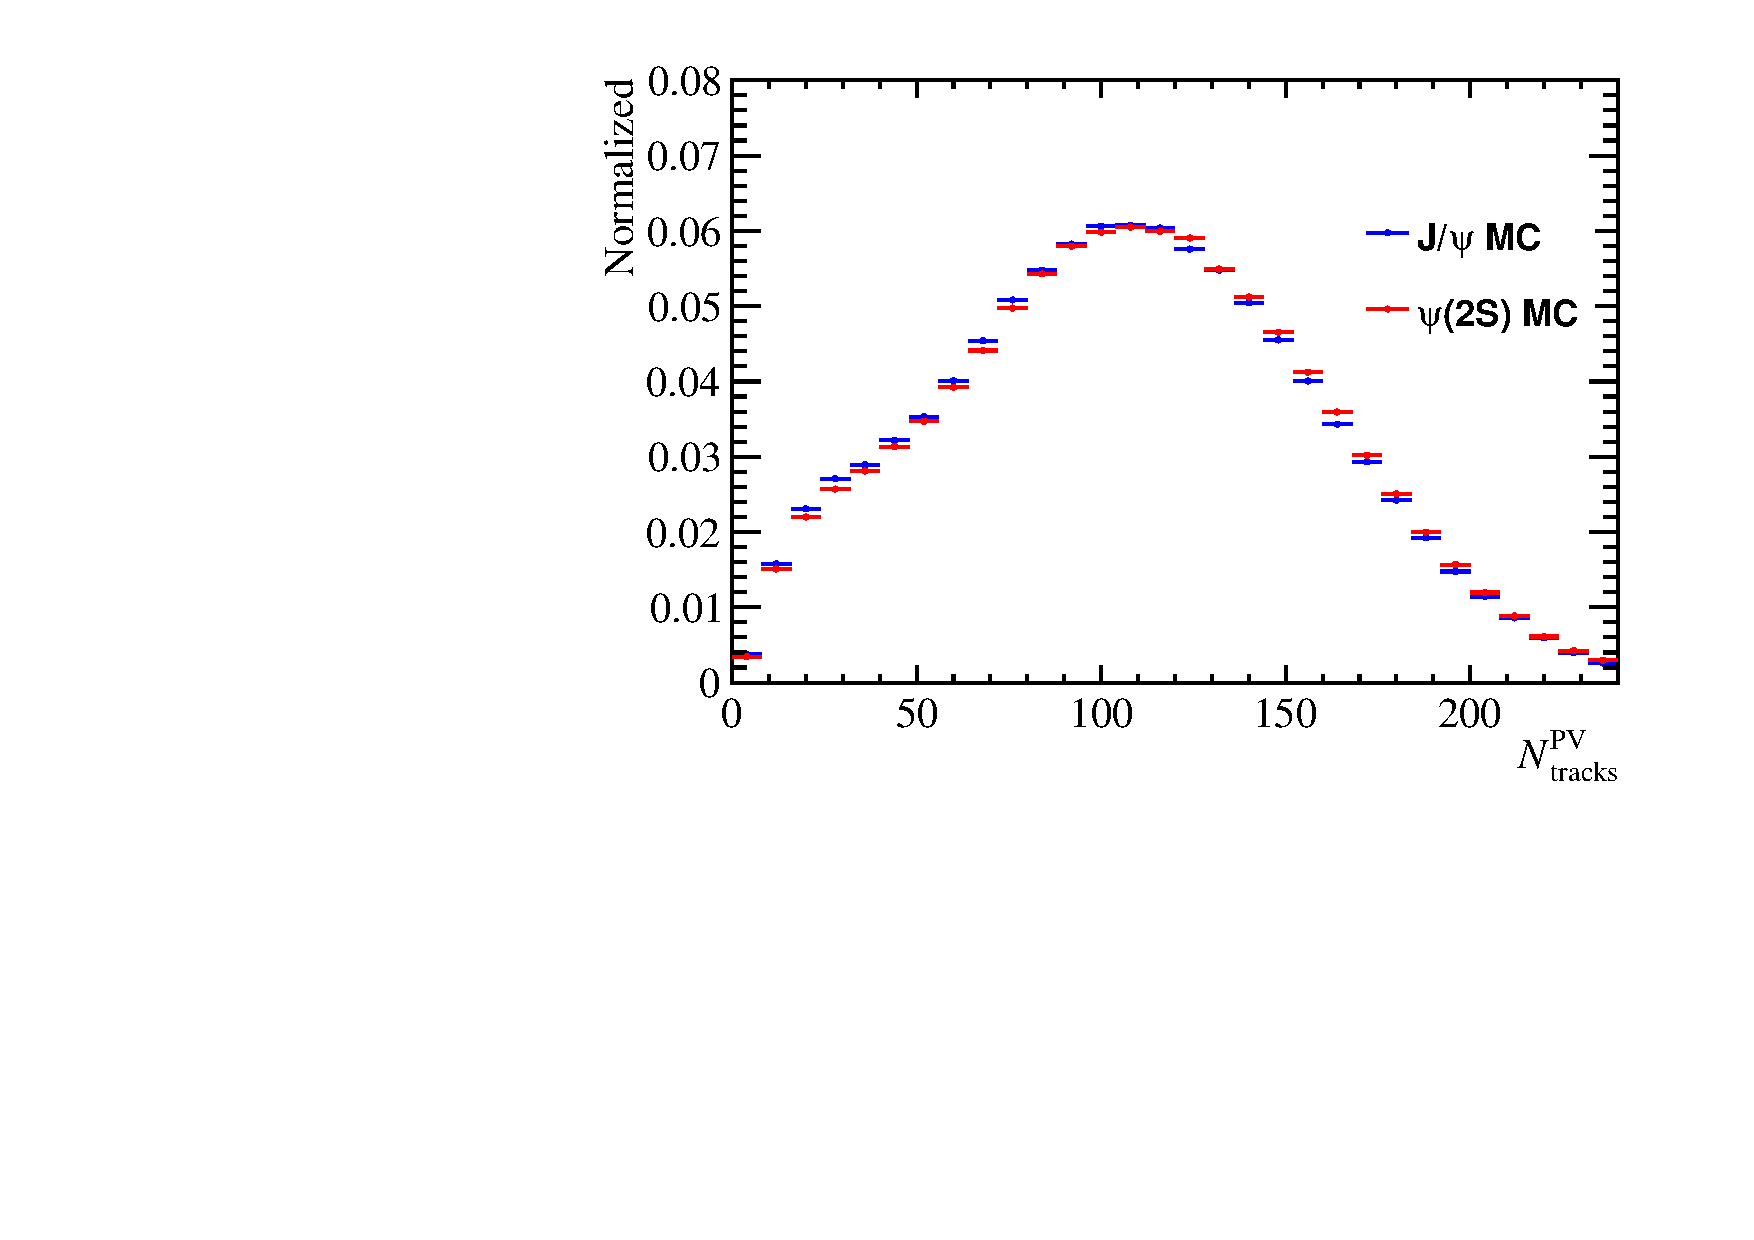
\includegraphics[width=0.32\linewidth]{pdf/pPb/Workdir/Reweight/MCMul.pdf}
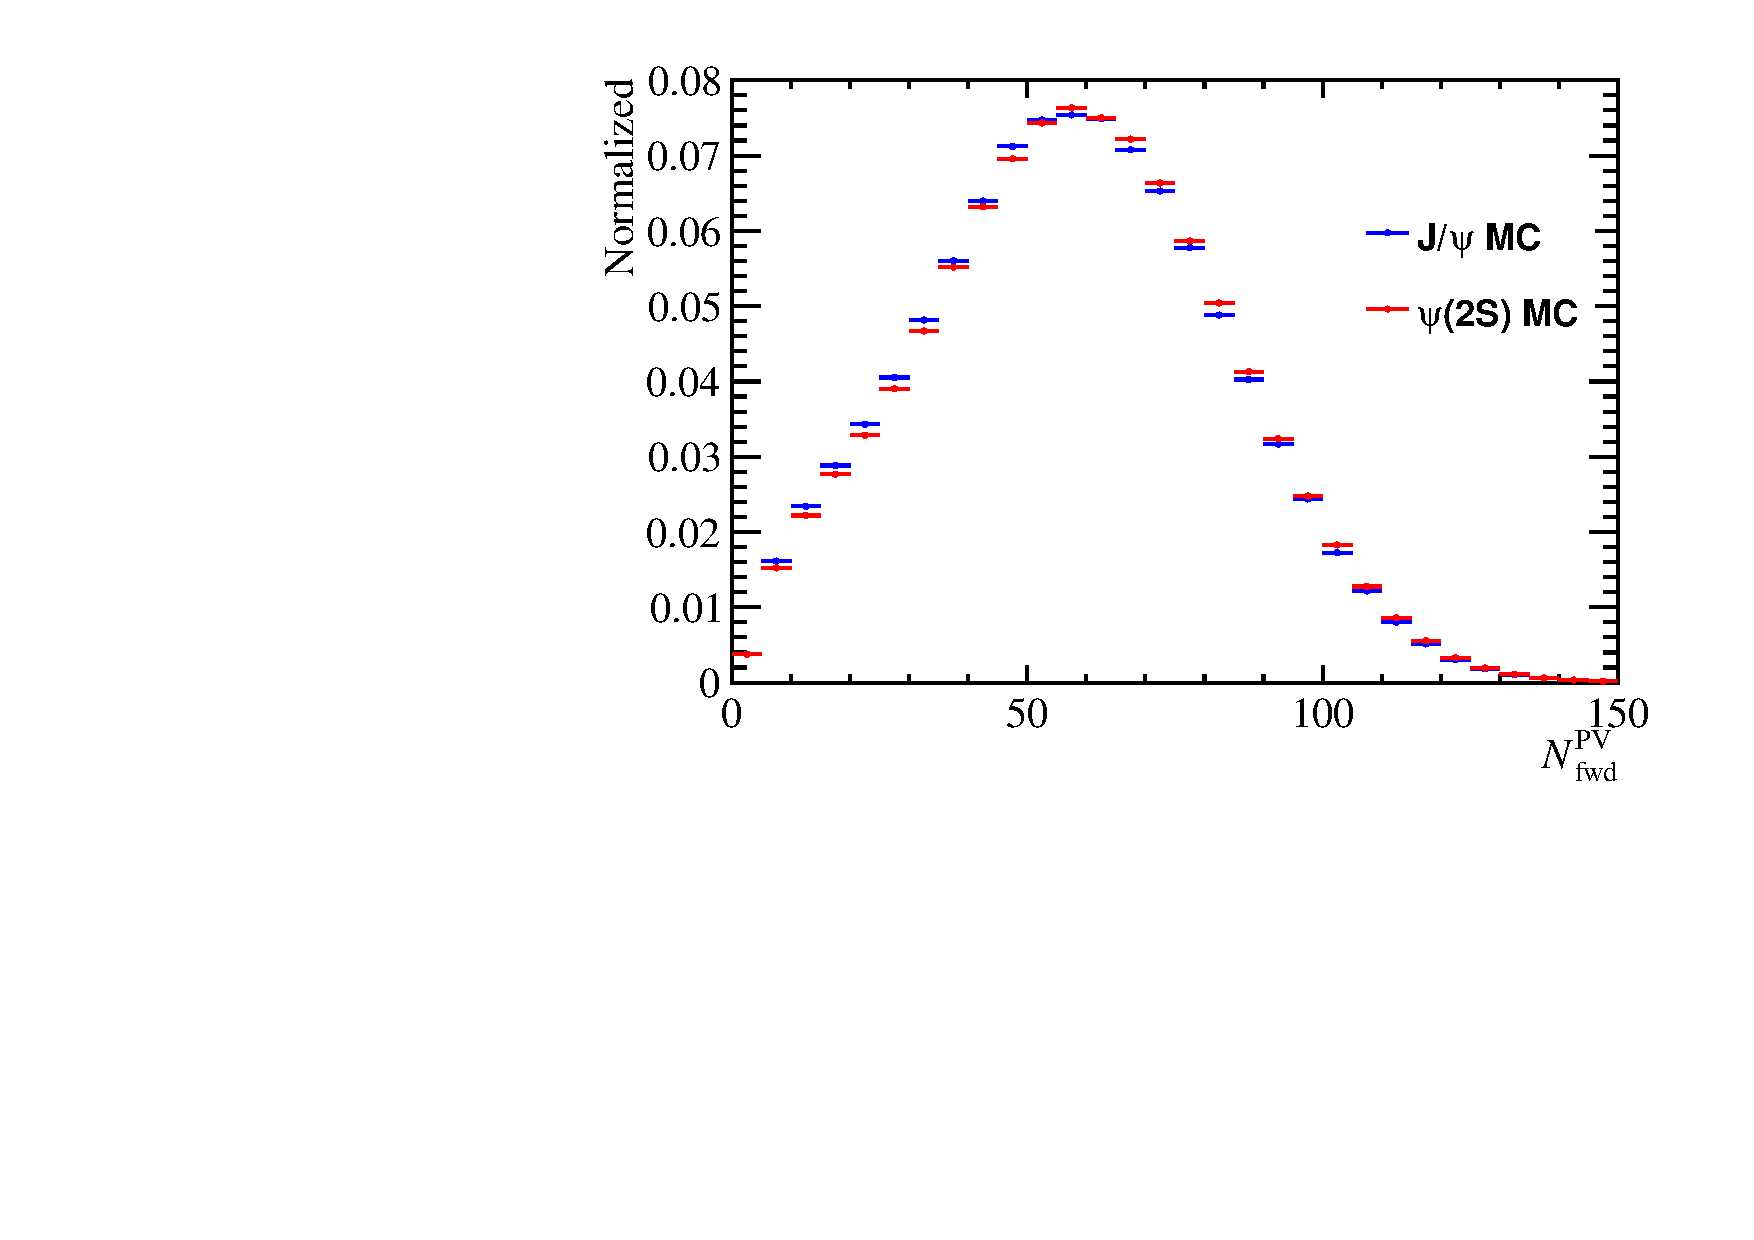
\includegraphics[width=0.32\linewidth]{pdf/pPb/FWorkdir/Reweight/MCMul.pdf}
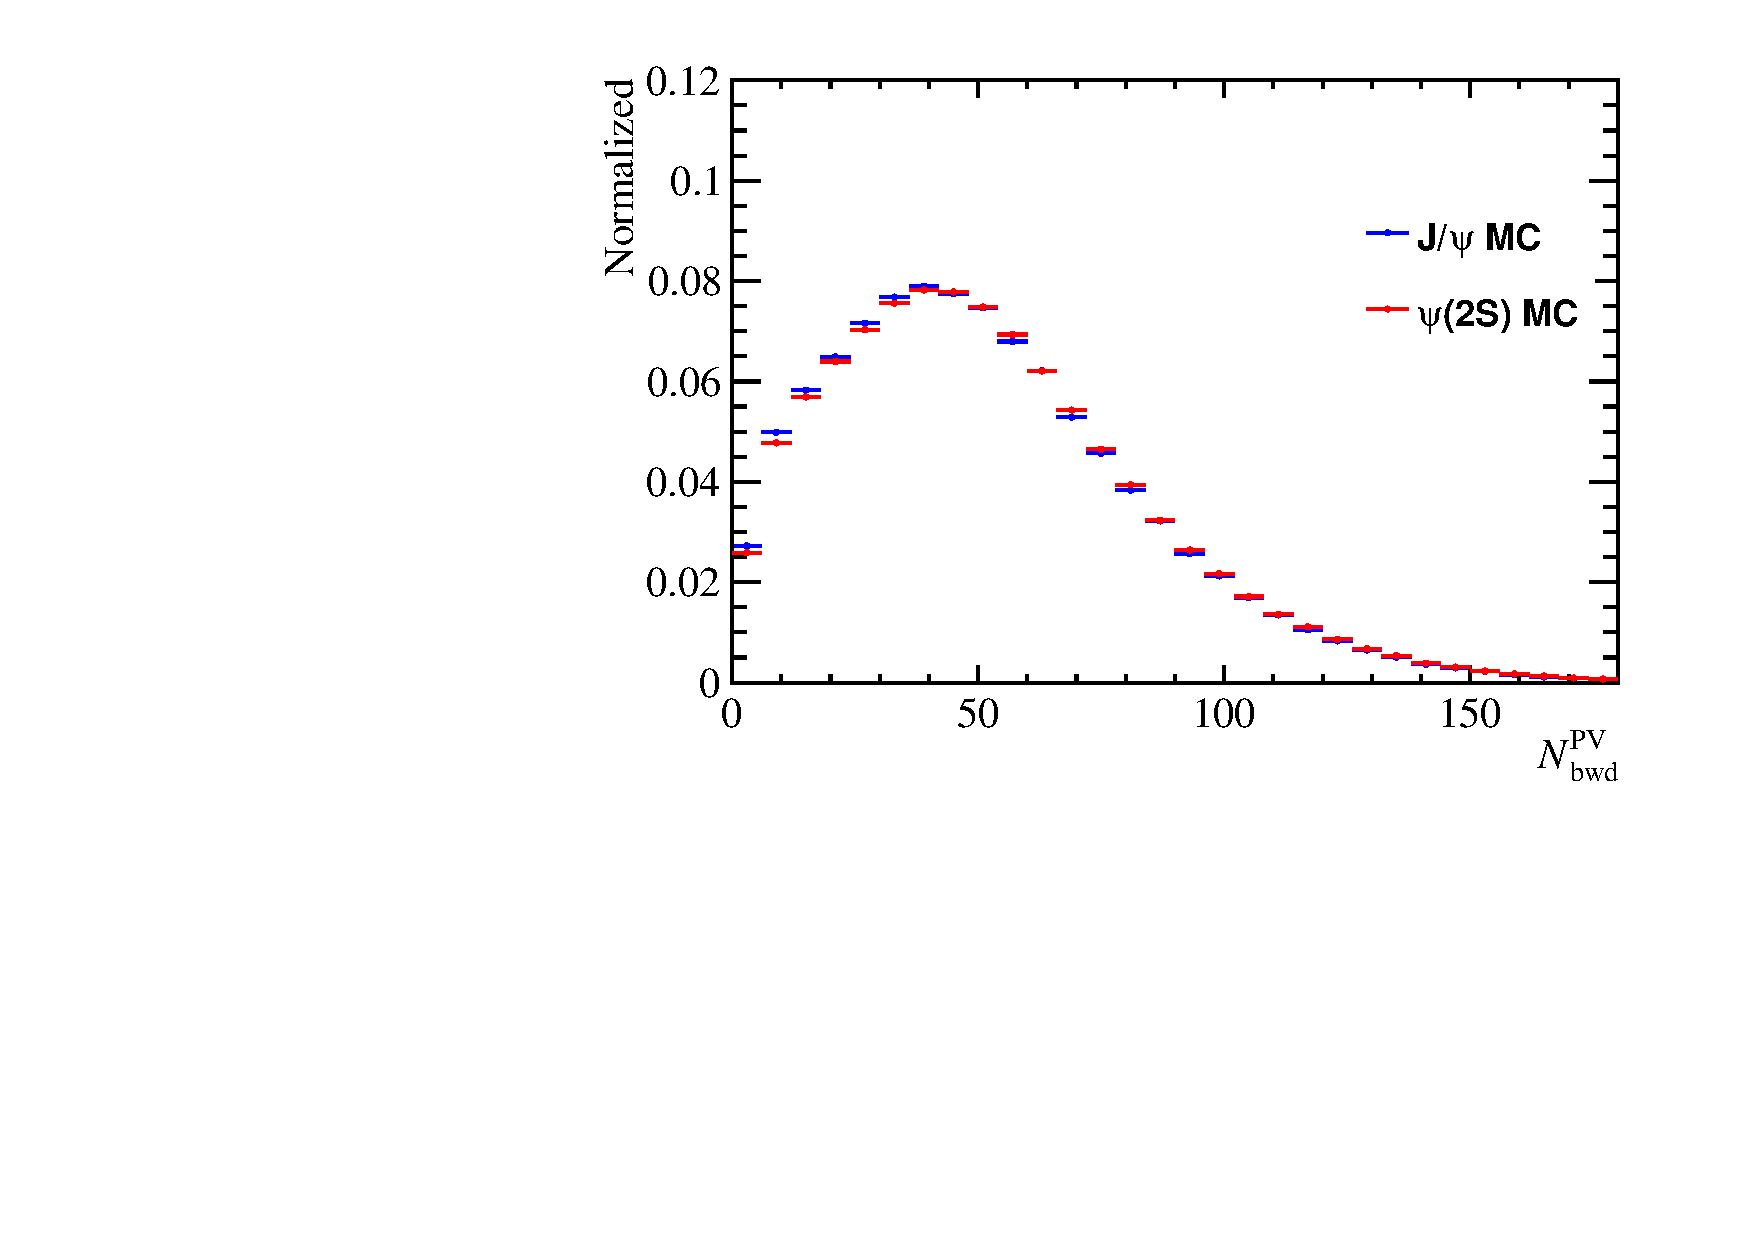
\includegraphics[width=0.32\linewidth]{pdf/pPb/BWorkdir/Reweight/MCMul.pdf}
\end{center}
\caption{
	Distribution of multiplicity variables for s-weight data (first row) and MC (second row) in $p$Pb configuration.}
\label{MulReweight}
\end{figure}

The difference in Monte Carlo sample and s-weight data for \jpsi and \psitwos should cancel. But the distribution of transverse momentum and rapidity in high- and low- multiplicity for both \jpsi and \psitwos is not negligible. So two samples of high- and low-multiplicity classes are considered when re-weighting Monte Carlo sample to match s-weight data (the high- and low-multiplicity samples are seperated by the mean values of multiplicity variables we choose accordingly). As an example, the re-weight of \pt and $y^*$ for high- and low-multiplicity \jpsi samples when taking $N_{\rm tracks}^{\rm PV}$ as multiplicity variable is shown in Figure~\ref{PTYReweightJ}. And that for \psitwos is shown in Figure~\ref{PTYReweightP}.
\begin{figure}[H]
\begin{center}
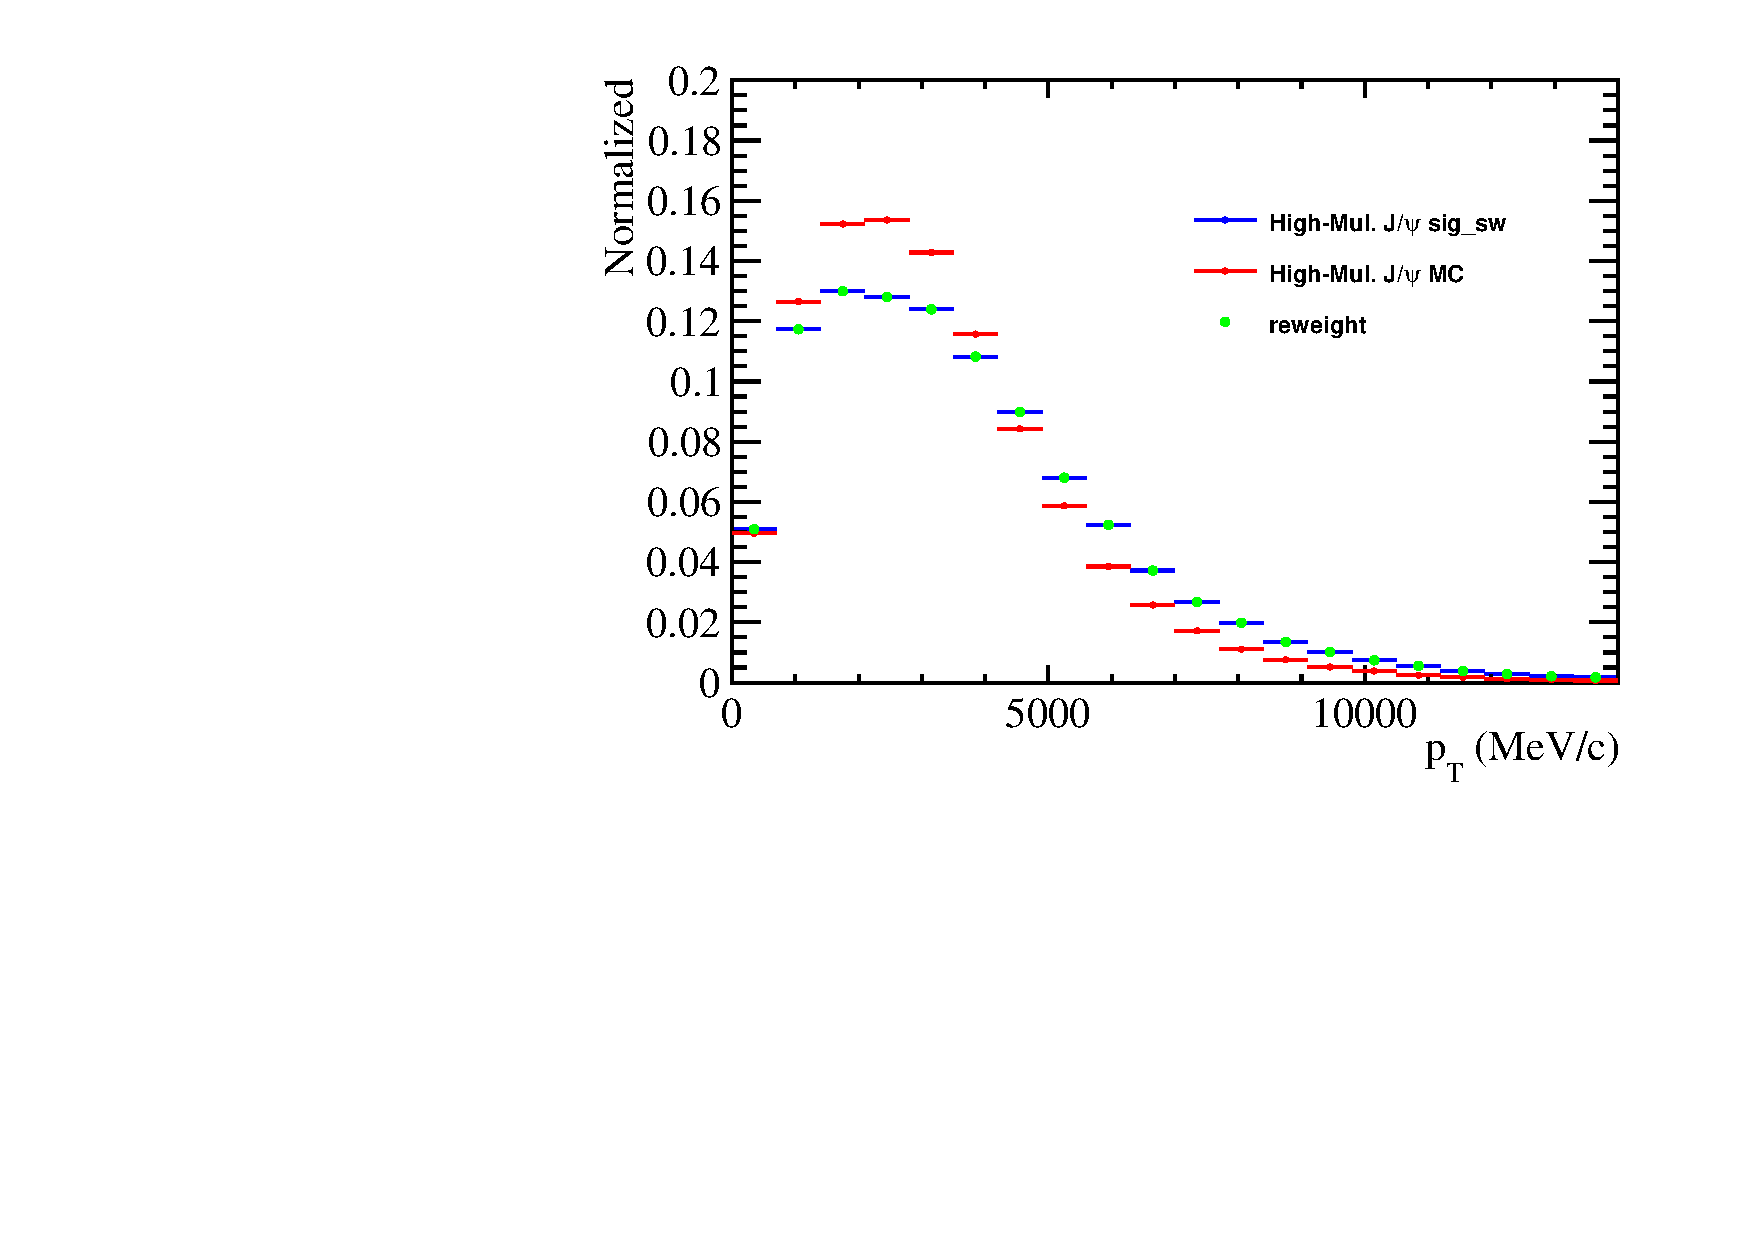
\includegraphics[width=0.37\linewidth]{pdf/pPb/Workdir/Reweight/JpsiHighMulPT.pdf}
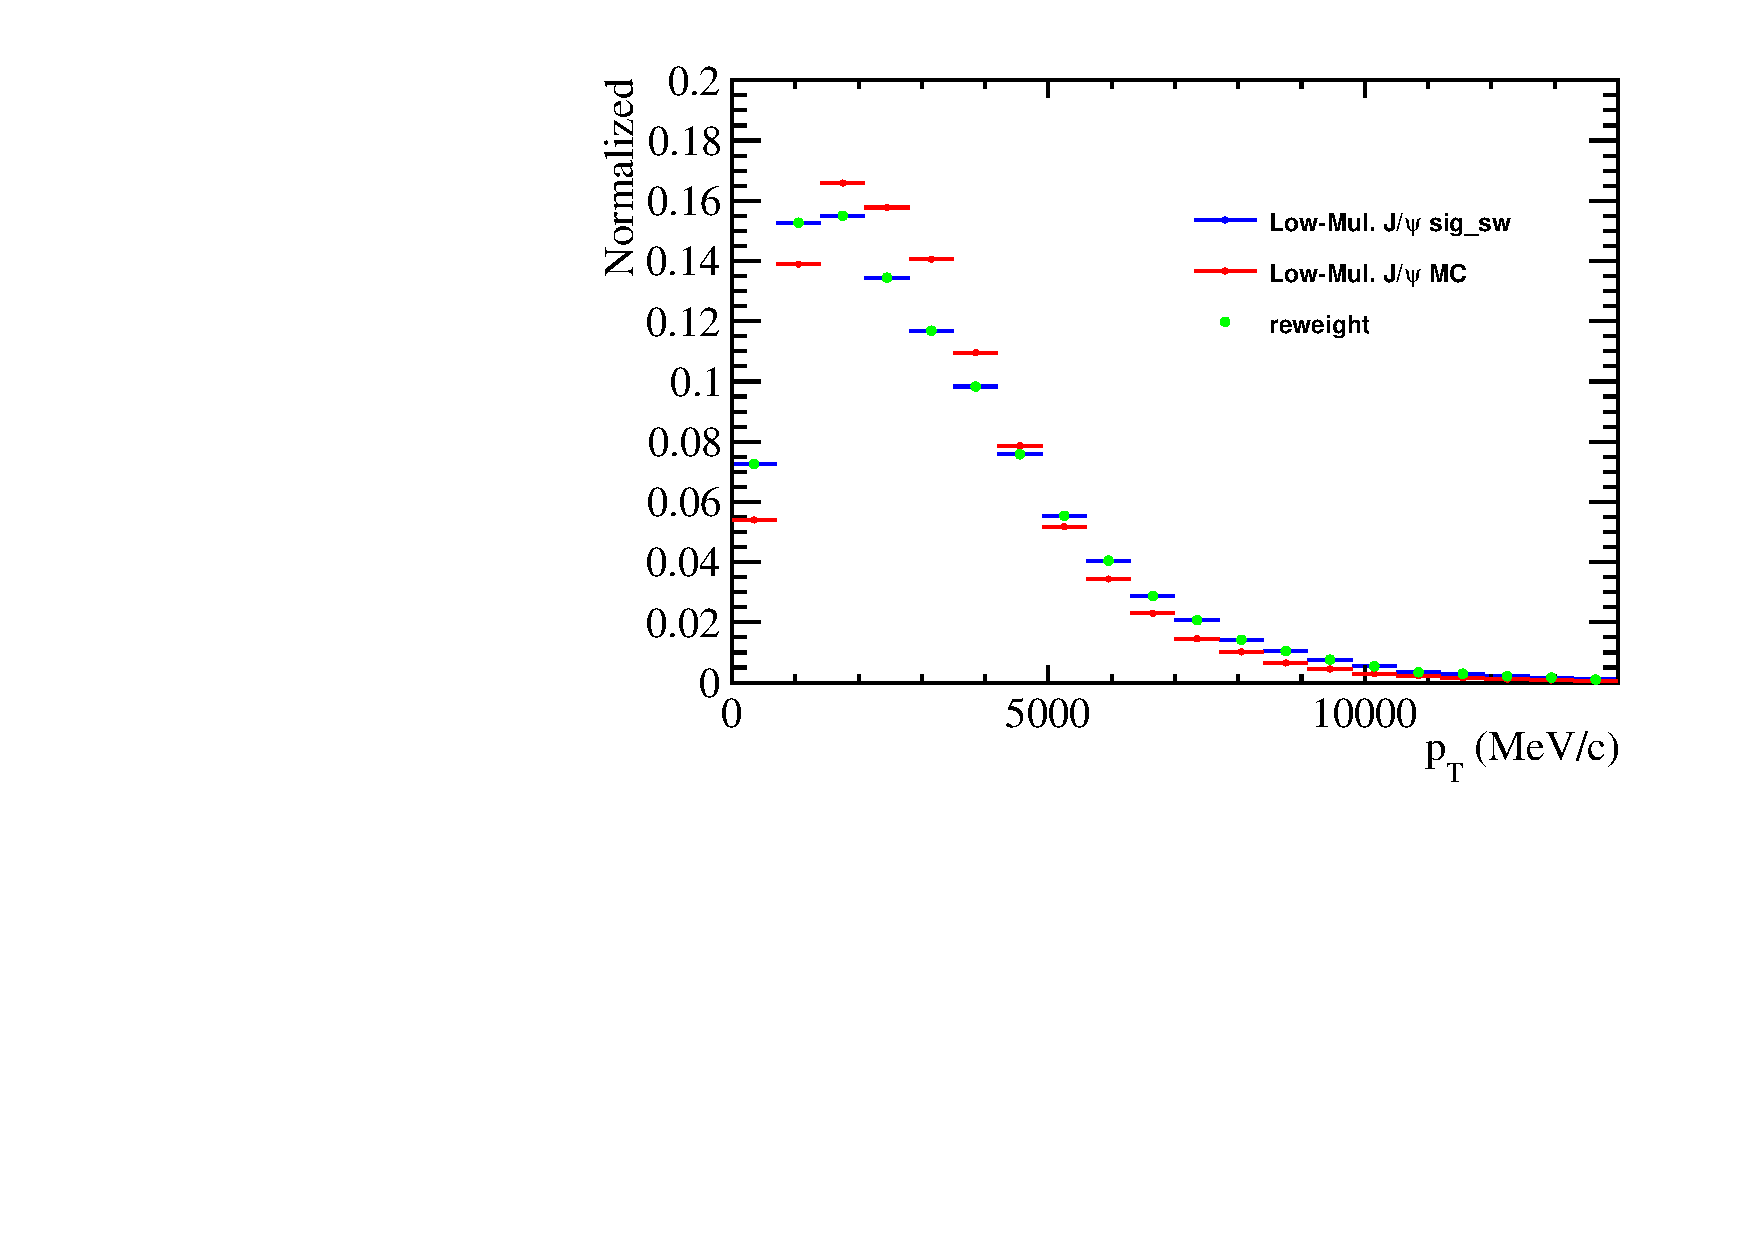
\includegraphics[width=0.37\linewidth]{pdf/pPb/Workdir/Reweight/JpsiLowMulPT.pdf}
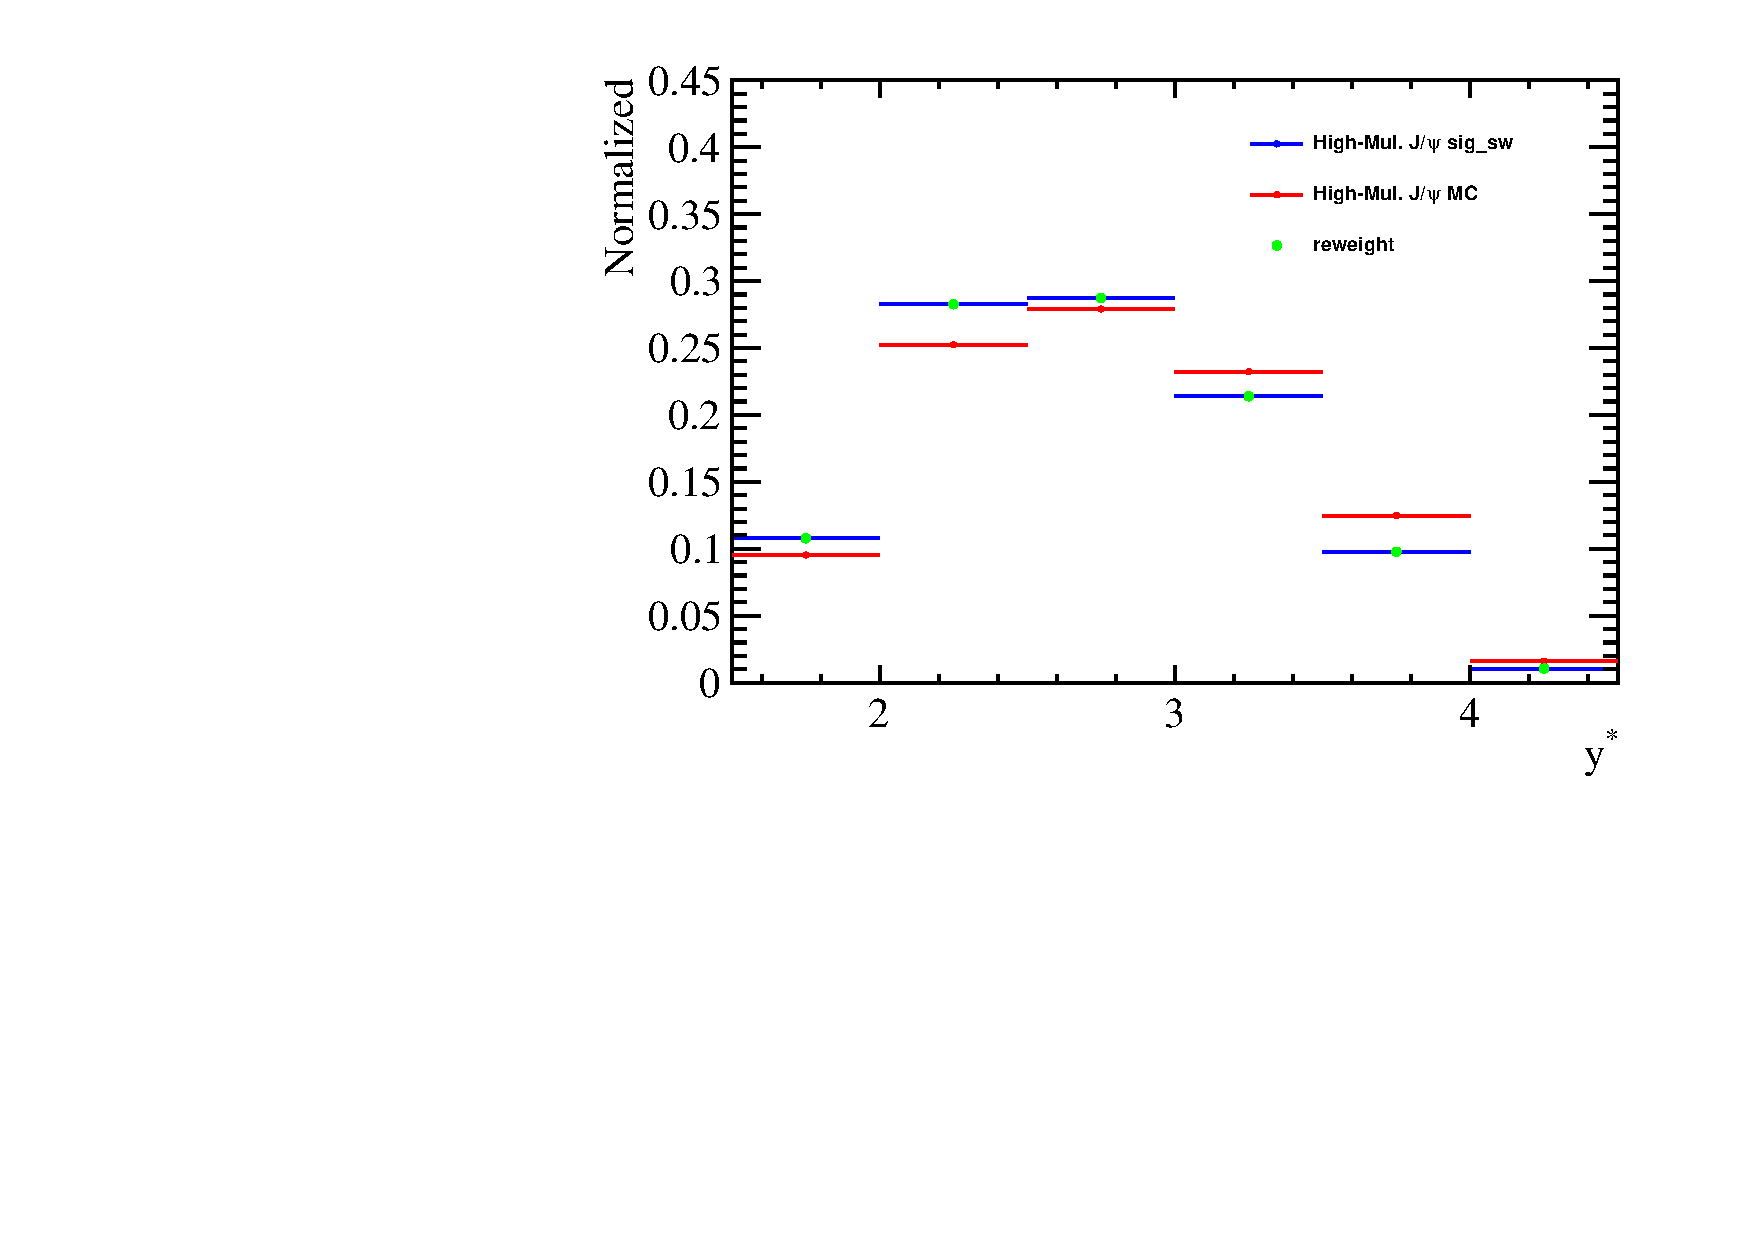
\includegraphics[width=0.37\linewidth]{pdf/pPb/Workdir/Reweight/JpsiHighMulY.pdf}
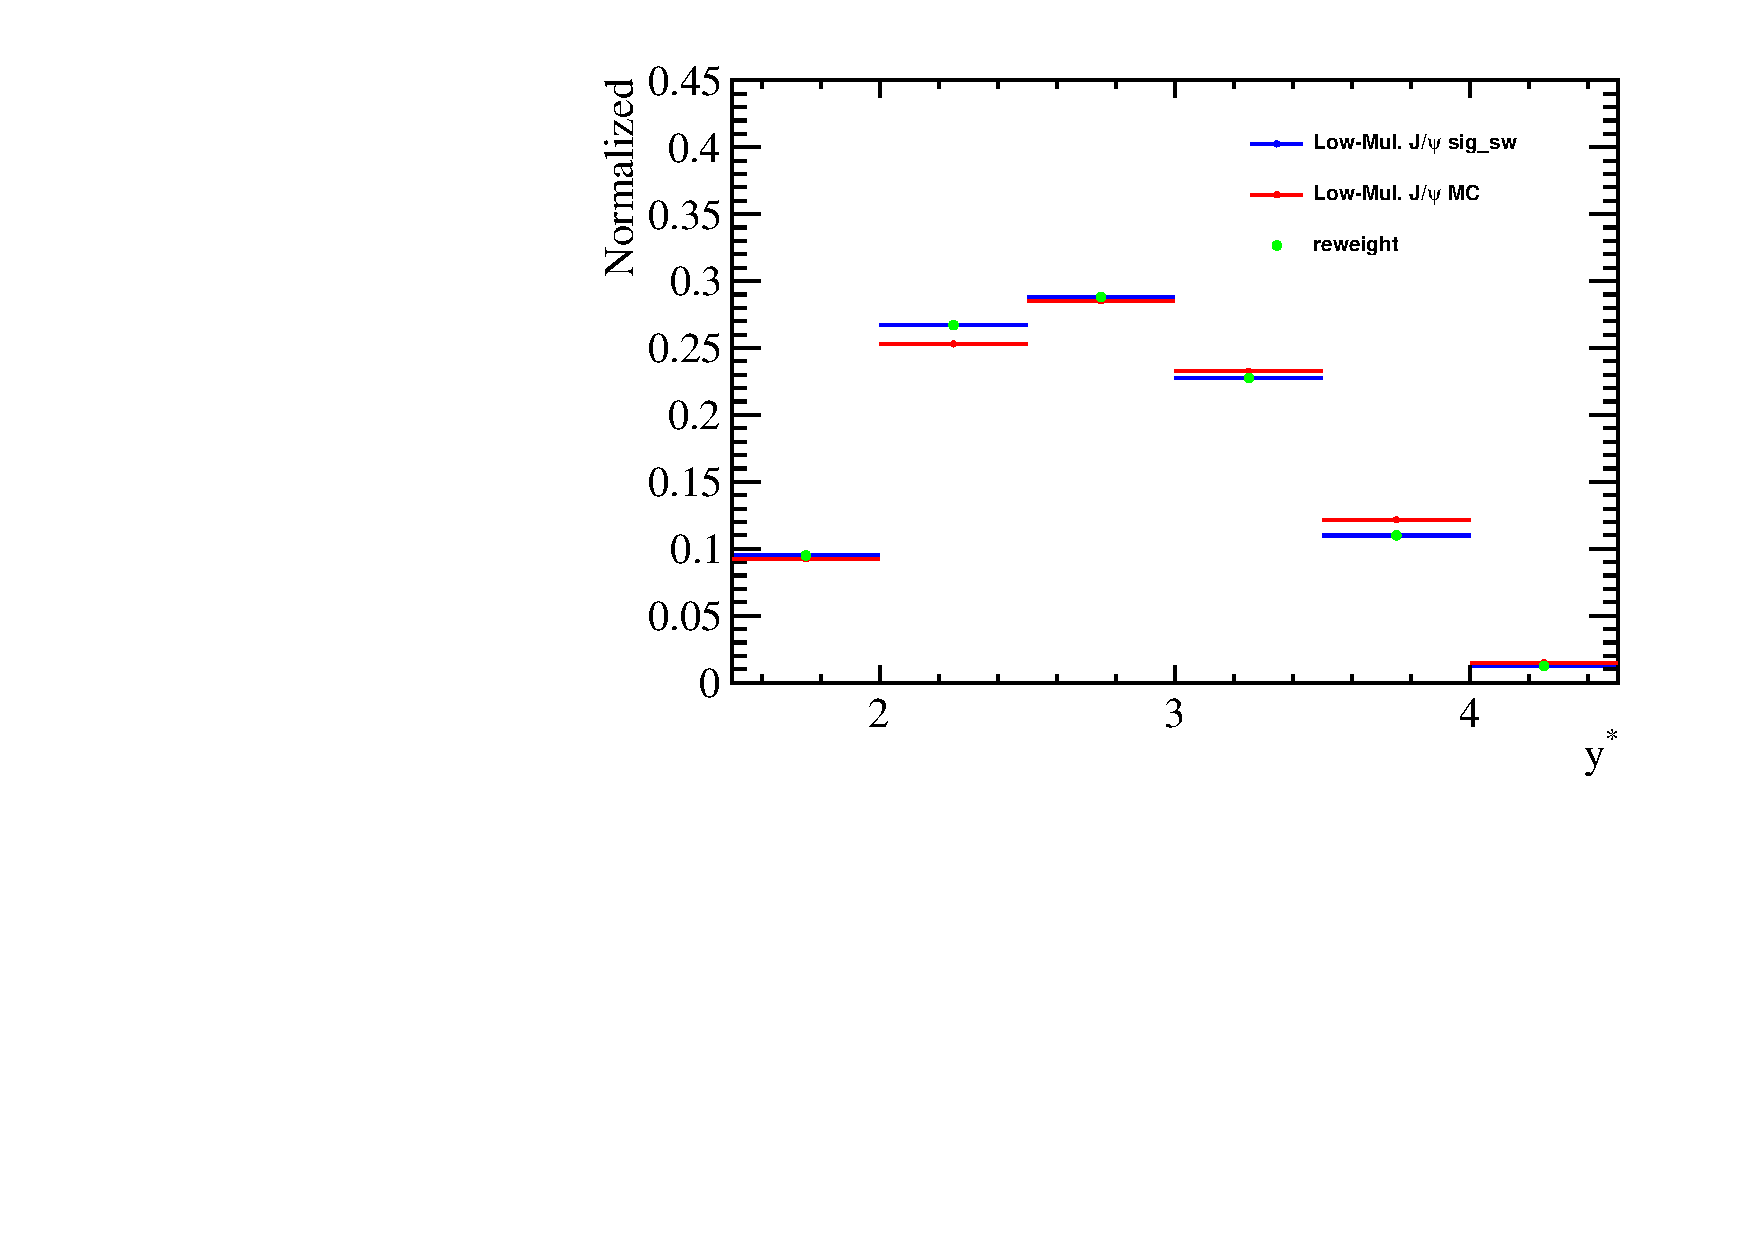
\includegraphics[width=0.37\linewidth]{pdf/pPb/Workdir/Reweight/JpsiLowMulY.pdf}
\end{center}
\caption{
        Re-weight of \pt (first row) and $y^*$ (second row) for high- (left) and low-multiplicity (right) \jpsi samples in $p$Pb configuration.}
\label{PTYReweightJ}
\end{figure}

\begin{figure}[H]
\begin{center}
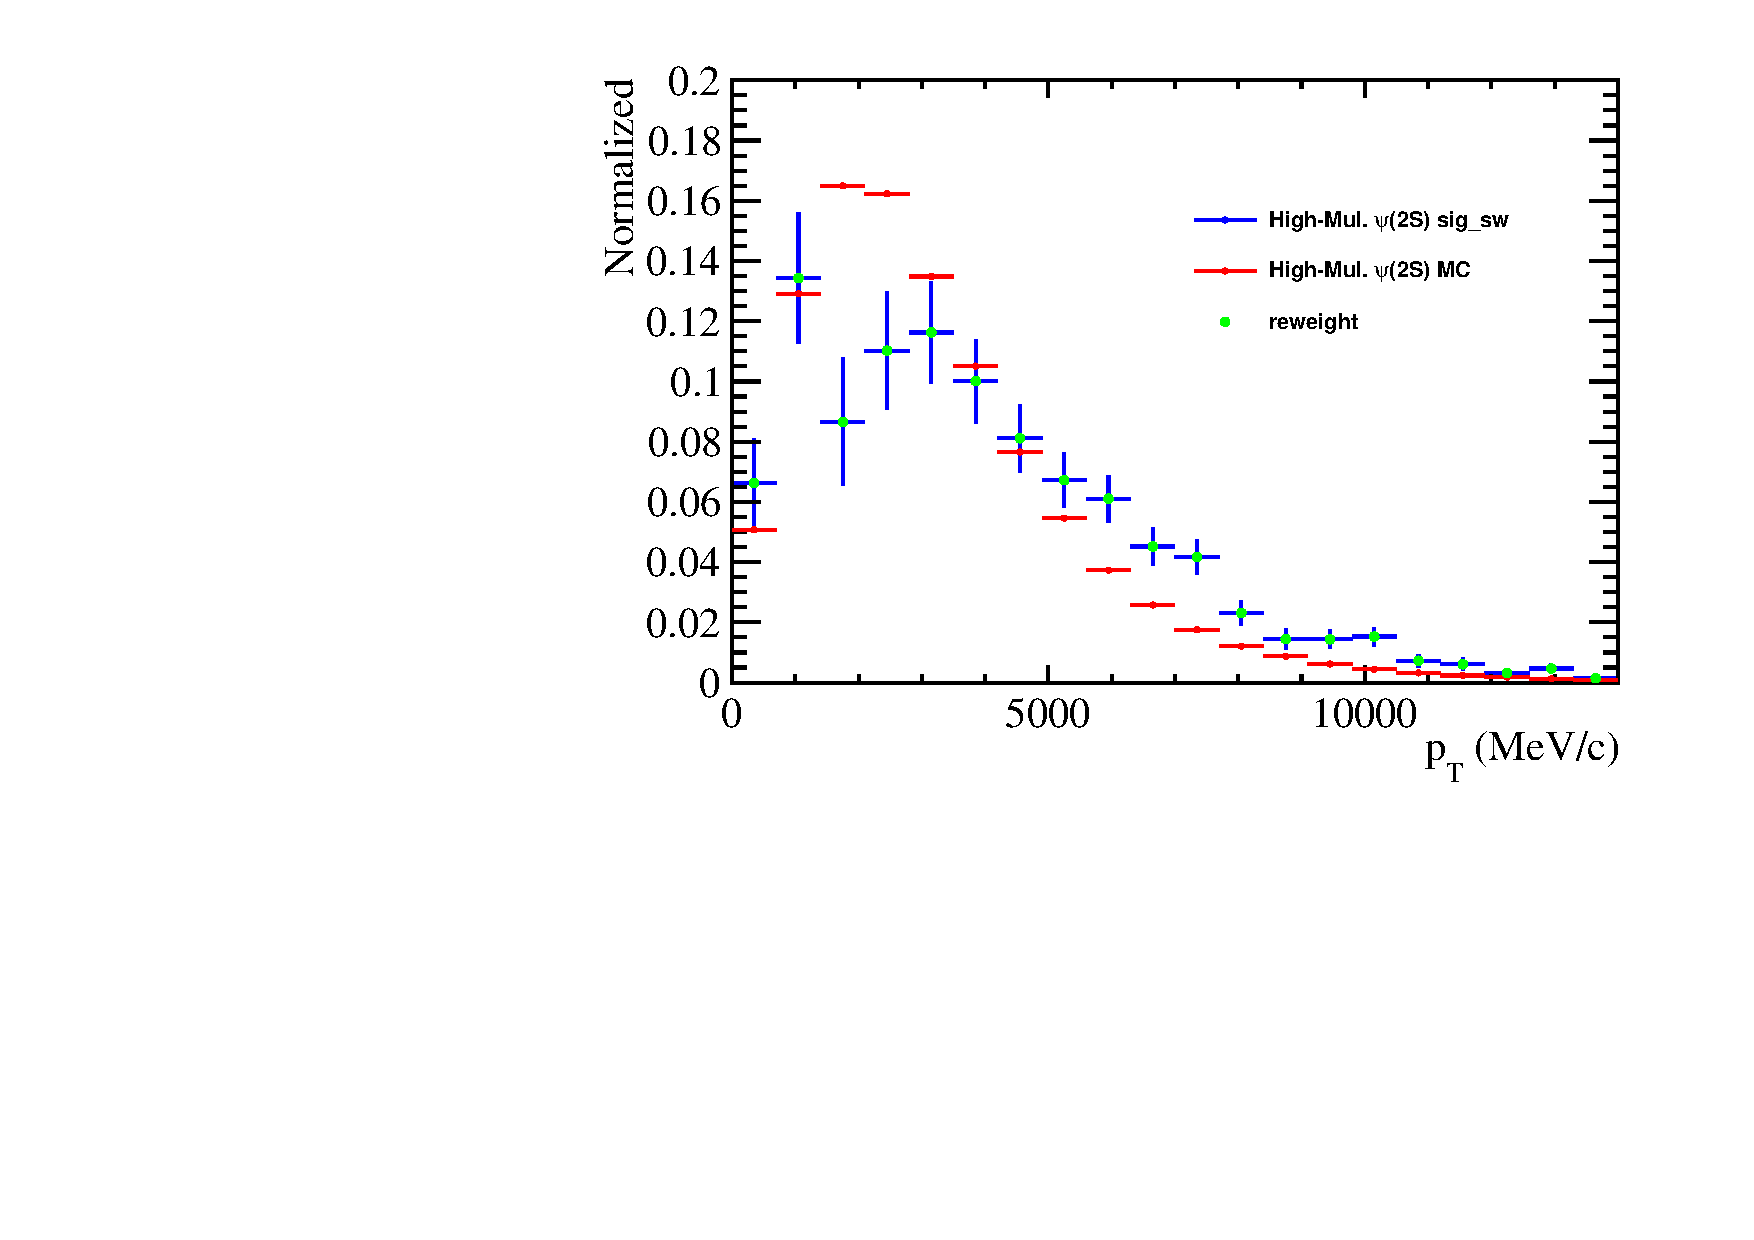
\includegraphics[width=0.37\linewidth]{pdf/pPb/Workdir/Reweight/Psi2SHighMulPT.pdf}
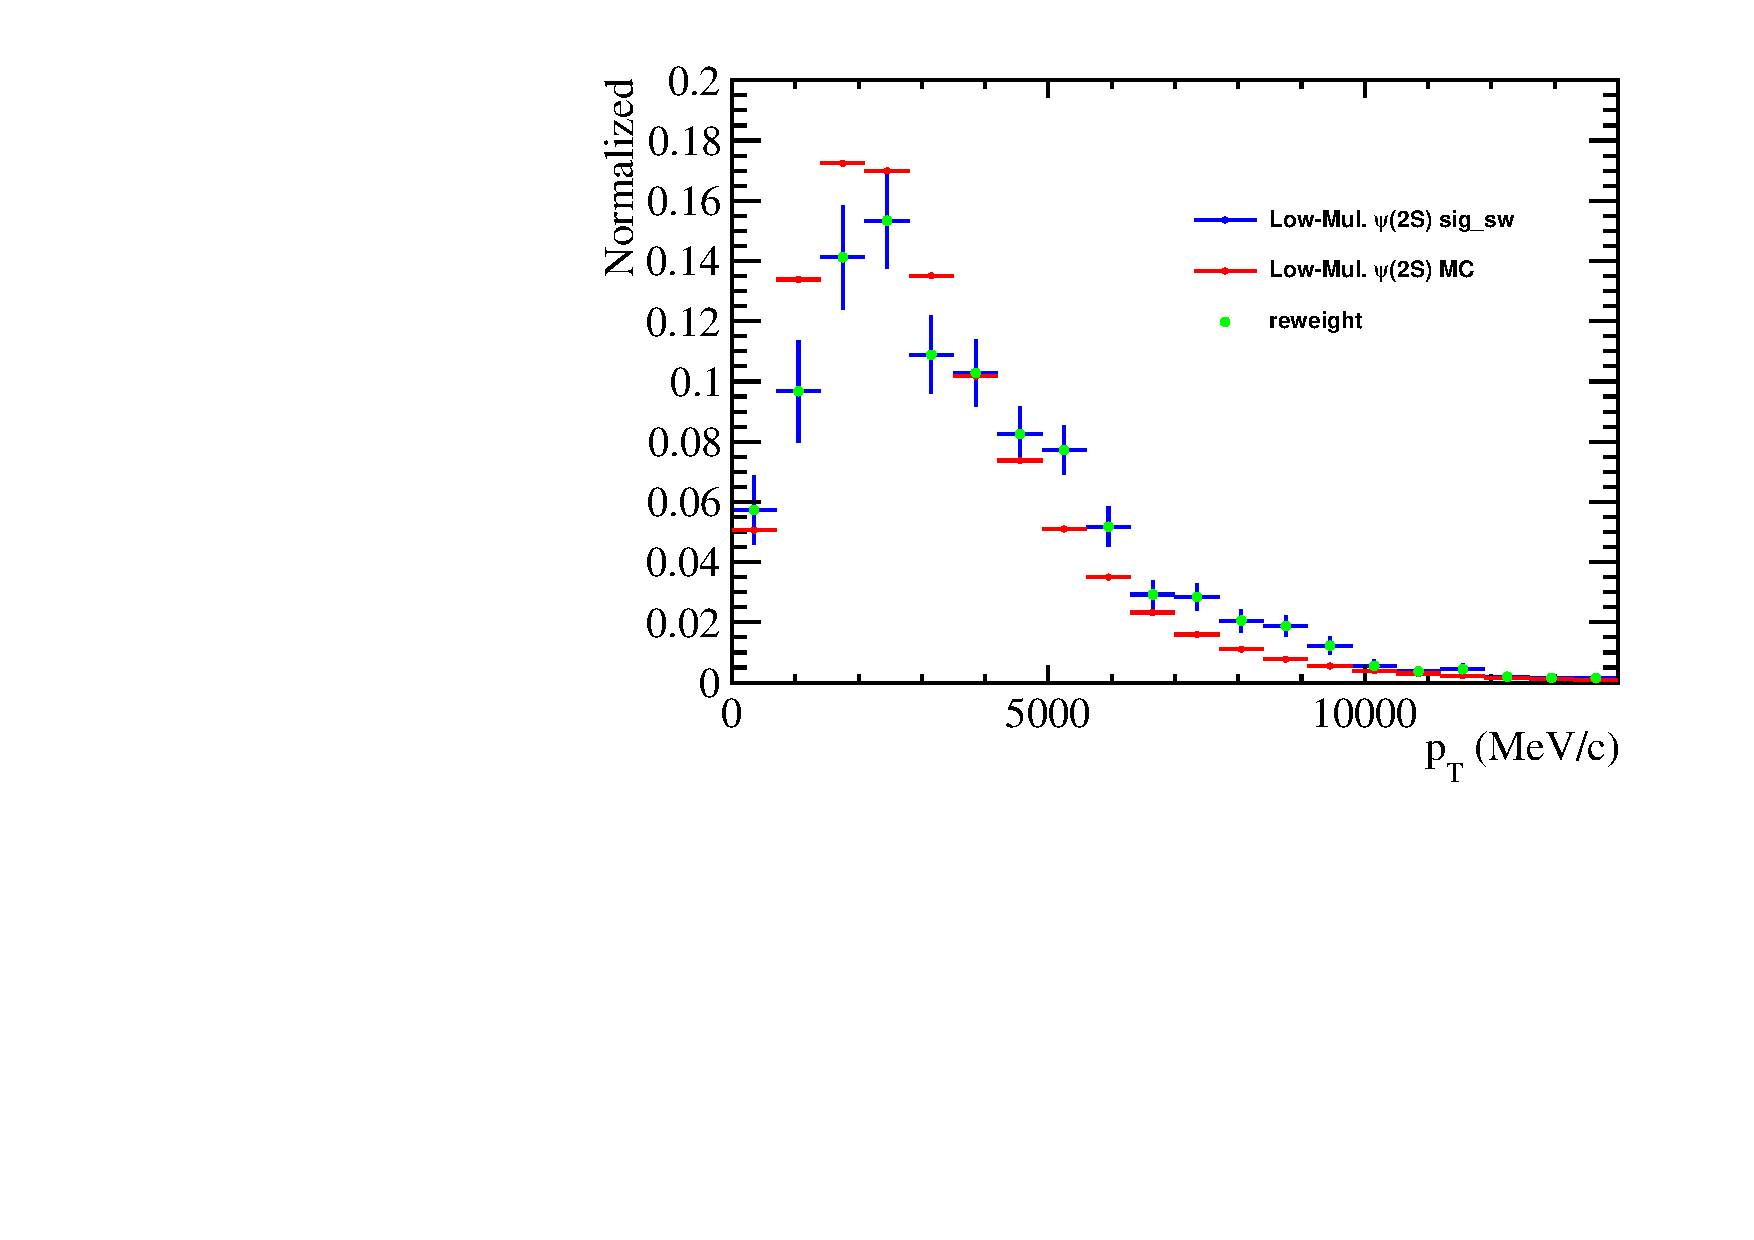
\includegraphics[width=0.37\linewidth]{pdf/pPb/Workdir/Reweight/Psi2SLowMulPT.pdf}
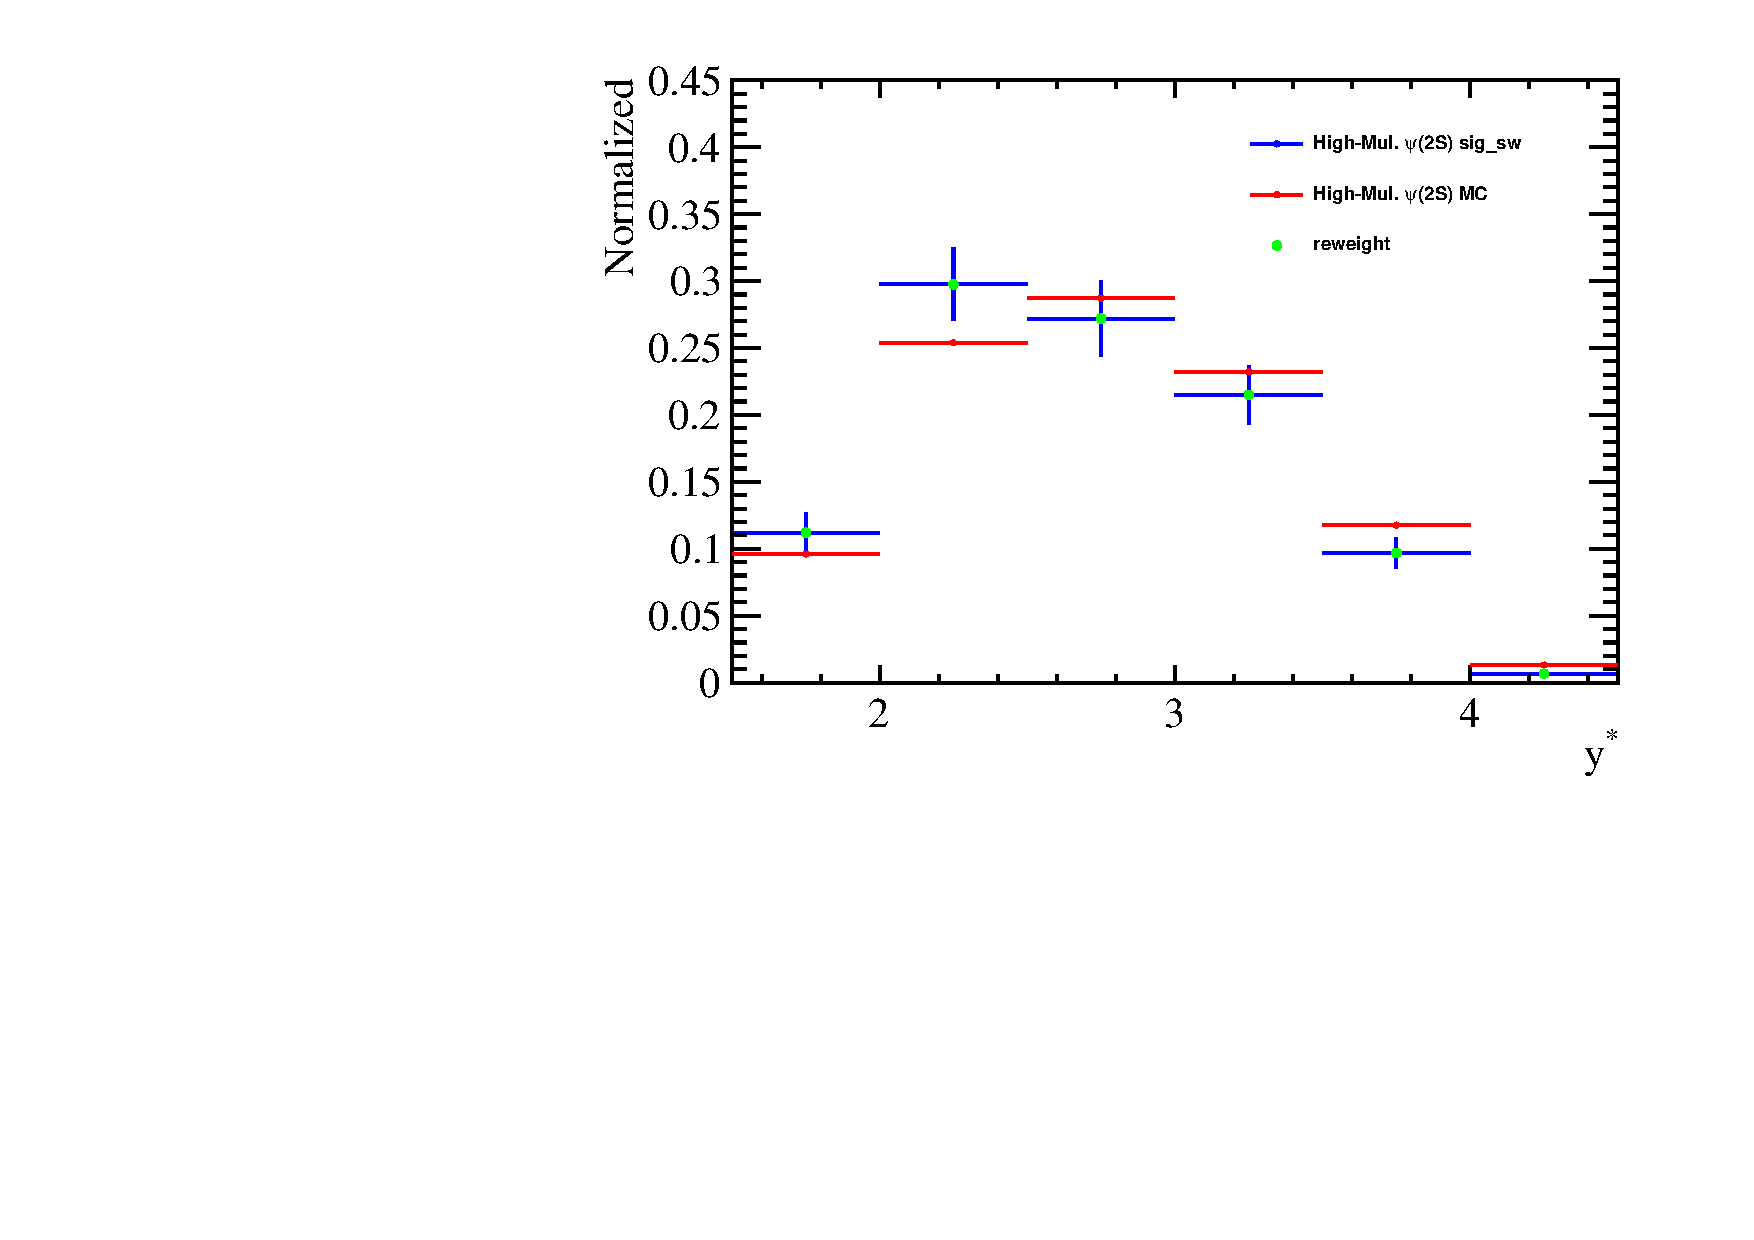
\includegraphics[width=0.37\linewidth]{pdf/pPb/Workdir/Reweight/Psi2SHighMulY.pdf}
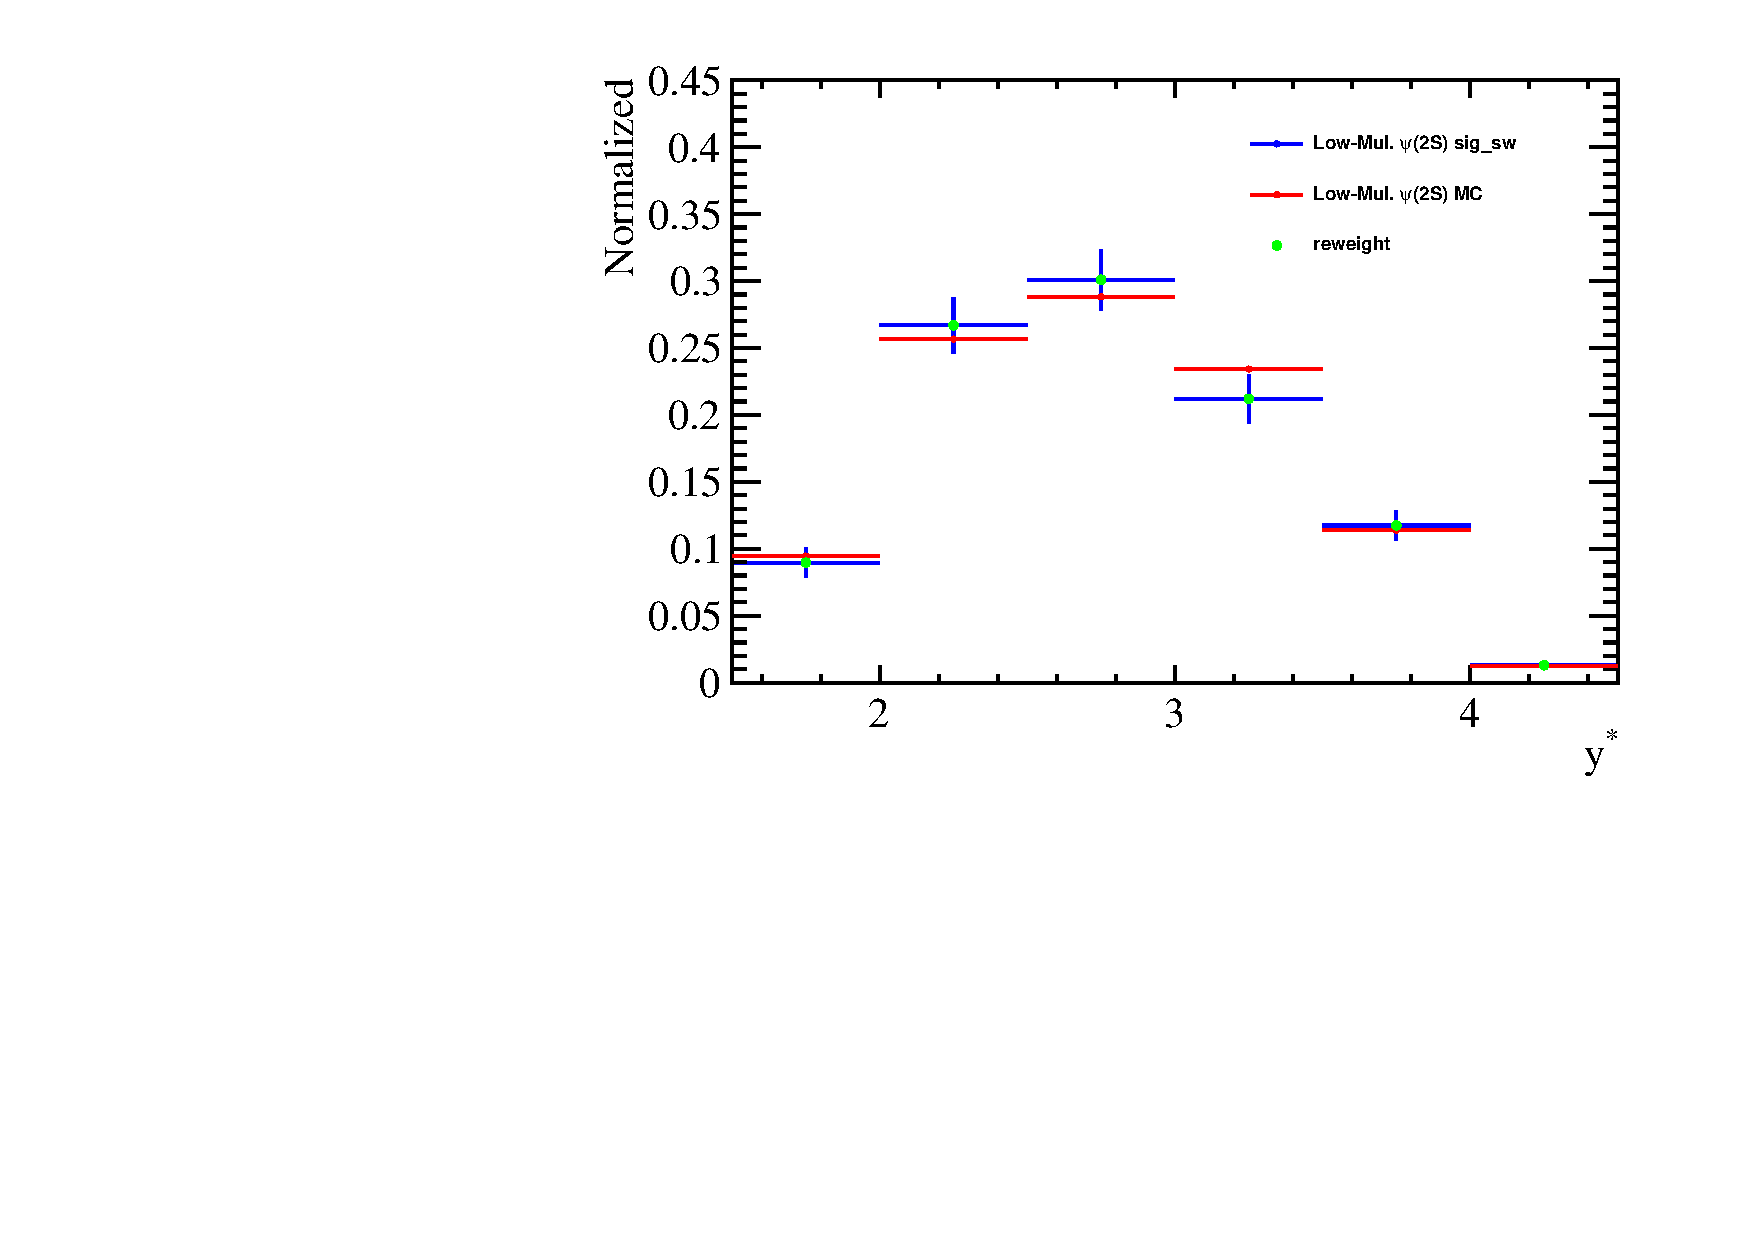
\includegraphics[width=0.37\linewidth]{pdf/pPb/Workdir/Reweight/Psi2SLowMulY.pdf}
\end{center}
\caption{
	Re-weight of \pt (first row) and $y^*$ (second row) for high- (left) and low-multiplicity (right) \psitwos samples in $p$Pb configuration.}
\label{PTYReweightP}
\end{figure}

\subsection{Acceptance}
The acceptance efficiency is defined as
\begin{equation}
    \effAcc(\pt,y^*)=\frac{\jpsi(\psitwos) \mathrm{ \ in \  bin \ } (\pt,y^*) \mathrm{ \ with  \ both \ } \mu \mathrm{ \ in \  LHCb \ }}{\jpsi(\psitwos) \mathrm{ \ generated \ in \ bin \ }(\pt,y^*)}
\end{equation}
 It is estimated from generator-level only simulations, using the settings described in Sect~\ref{Data and Monte Carlo samples}. Both $\mu$ in LHCb means here that they have a pseudo-rapidity $\eta$ between 2 and 5, before the magnet. In this analysis we only care about the ratio of acceptance efficiencies $R_{acc}$. When calculating the ratio of acceptance efficiencies, 50 random re-weight tables of \pt and $y^*$ from high- and low-multiplicity samples are generated (100 in total) for both \jpsi and \psitwos, within each bin a Gaussian random number is generated with mean the content and sigma the uncertainty. Then the 100 tables are introduced as correction to acceptance efficiencies. Then 100 ratios of acceptance efficiencies are calculated. Fit 100 $R_{acc}$ values with a Gaussian function we get the mean value as the ratio of acceptance efficiencies and the sigma be its systematic uncertainty. As an example, the fit result for $R_{acc}$ when global cuts for $N_{\rm tracks}^{\rm PV}$ as multiplicity are applied is shown in Figure~\ref{EffAccRatio}. The value is as follows,
\begin{equation}
	R_{acc}=\frac{\ensuremath{\epsilon_{\mathrm{acc,\jpsi}}}}{\ensuremath{\epsilon_{\mathrm{acc,\psitwos}}}}=0.991\pm 0.012.
\end{equation}
\begin{figure}[H]
\begin{center}
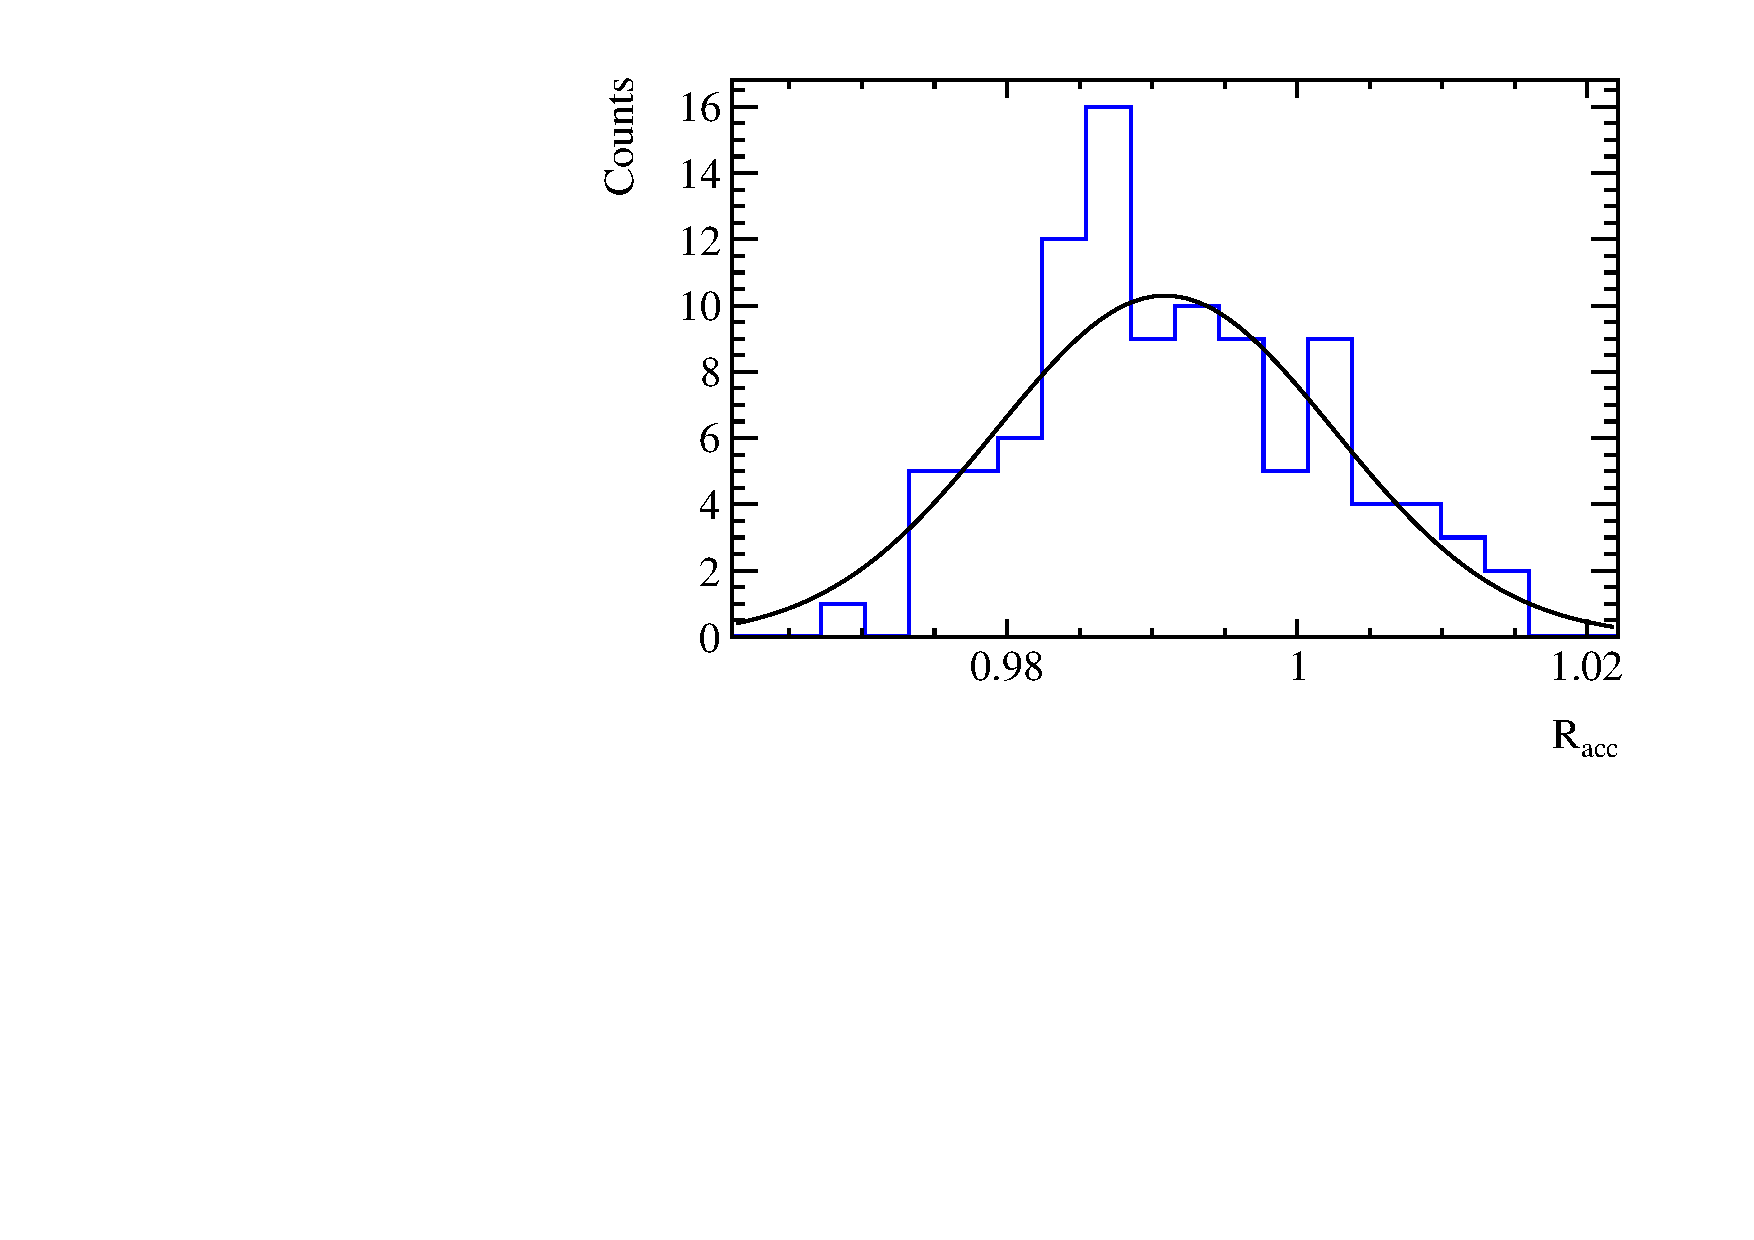
\includegraphics[width=0.5\linewidth]{pdf/pPb/Workdir/Eff_RecselPIDTrigger/Racc.pdf}
\end{center}
\caption{
	Fit Gaussian function on the distribution of $R_{acc}$ from 100 trials with global cuts for $N_{\rm tracks}^{\rm PV}$ as multiplicity variable.}
\label{EffAccRatio}
\end{figure}


 \subsection{Reconstruction and selection efficiency}
 The reconstruction and selection efficiency is defined as the fraction of \jpsi (\psitwos) in the acceptance, where both muons are reconstructed as long tracks and then pass the offline selections,
 \begin{equation}
    \effReco(\pt,y^*)=\frac{\jpsi(\psitwos) \mathrm{ \ in \  bin \ } (\pt,y^*) \mathrm{ \ with  \ both \ } \mu \mathrm{ \ reconstructed \ and \ selected}}{\jpsi(\psitwos) \mathrm{ \ in \  bin \ } (\pt,y^*) \mathrm{ \ with  \ both \ } \mu \mathrm{ \ in \  LHCb \ }}.
\end{equation}
%The tracking efficiency is computed using the simulation samples, and this efficiency is corrected using the reconstruction efficiency per-track estimated in data. The long method with tag-probe strategy for tracking efficiency calibration is implemented. In this method, a probe track is reconstructed only with hits in the TT and MUON stations. This probe muon track is combined with a standard long muon track to form a \jpsi candidate, and these candidates build a “pre-matched” sample. This standard long track has the same reconstruction algorithm as the signal tracks in our analysis, so they have the same tracking efficiency when they are in the same phase space. 
An additional standard long track, identified as a muon and with the same charge as the probe track, is combined with the \jpsi in the ”pre-matched” sample to form a good vertex. If this third track shares with the probe track more than $40\%$ of the hits in both the TT and MUON stations, the probe track is referred to as “matched”. The \jpsi candidates in the ”pre-match” sample that have the probe track matched, form the ”matched” sample. 
The tracking efficiency is computed as the matching efficiency, which is the fraction of probe tracks that match standard long tracks. The number of signal probe tracks and those matched to long tracks are estimated from the number of \jpsi signal candidates, measured by fitting to the $\mu^+\mu^-$ invariant mass distribution in the ”pre-matched” sample and the ”matched” sample, respectively. The reconstruction of the probe tracks, of the \jpsi candidates and the implementation of the matching are done at the trigger (HLT) level, available in both pp and proton-lead data. The relevant trigger lines are called $\textbf{Hlt2TrackEffDiMuonMuonTT(Minus|Plus)^*}$ (which selects the “pre-matched” samples), where Plus (Minus) means that the $\mu^+(\mu^-)$ is the probe track. These calibration events are processed via the TurboCalib stream. Due to higher multiplicity in proton-lead data, especially in the backward configuration, additional offline selections are applied to the \jpsi candidates out of TurboCalib stream. The tag track of the \jpsi candidates is required to have a good muon-pion separation with $PID(\mu)$ > 3, and the probe track is required to have a better fit quality with $Prob(\chi_{trk}^2) > 0.2$. The effect of these extra selections is studied with the proton-lead forward data sample ($p$Pb), where a better signal purity is obtained. 
Simulated \jpsi samples are produced with the same trigger processing as data for the calibration. The reconstruction software is identical to those used to reconstruct the simulated signals used in the analysis. 
The signal extraction fits to the mass distributions are implemented in bins of $\eta$ and $p$ of the probe tracks, allowing to determine the track reconstruction efficiency in the same bins. The bin boundaries are 1.9, 3.2 and 5.0 for $\eta$ and 6, 10, 20, 40, 100 and 500 $\gevc$ for $p$. No binning in detector occupancy is implemented due to limited statistics. However, since for both data and simulation, the occupancy distribution in the analysis samples and the calibration samples are consistent with each other,  the binning in detector occupancy is not necessary. 
The $\mu^+$ and $\mu^-$ probe tracks are fit separately. Thus for each kinematic bins, there are eight fits: $\mu^+$ or $\mu^-$ as the probe track; in the ”pre-matched” or ”matched” sample; for $p$Pb or Pb$p$. For the fits, the same signal shape is used for bins of the same $(p, \eta)$ interval: a Gaussian function plus a Crystal Ball function. The background is described by an exponential function. 
The procedure performed on data is applied identically to the $p$Pb and Pb$p$ simulation calibration samples. The tracking efficiencies for $\mu^+$ and $\mu^-$ are averaged, as for the cross-section measurements charge conjugated states are added together.
Finally, we calculate the ratio of single track reconstructions efficiencies between data and simulation. The results are given in Figure~{TrackTable}. The corresponding uncertainty for each value is also shown. The ratio reconstruction and selection efficiency is then computed from the full simulation, and correcting the efficiency using the per-track efficiency ratios detailed above.
Then the reconstruction efficiency is further corrected using the data-over-simulation single tracking efficiency ratio. The ratio of tracking efficiencies for a single track in data and simulation determined with the Long Tag-Probe method is shown in Figure~\ref{TrackTable} which was given by the tracking group. For a given event the correction factor is determined by multiplying the efficiency ratios for each of the tracks in the final state.
\begin{figure}[!tbp]
\begin{center}
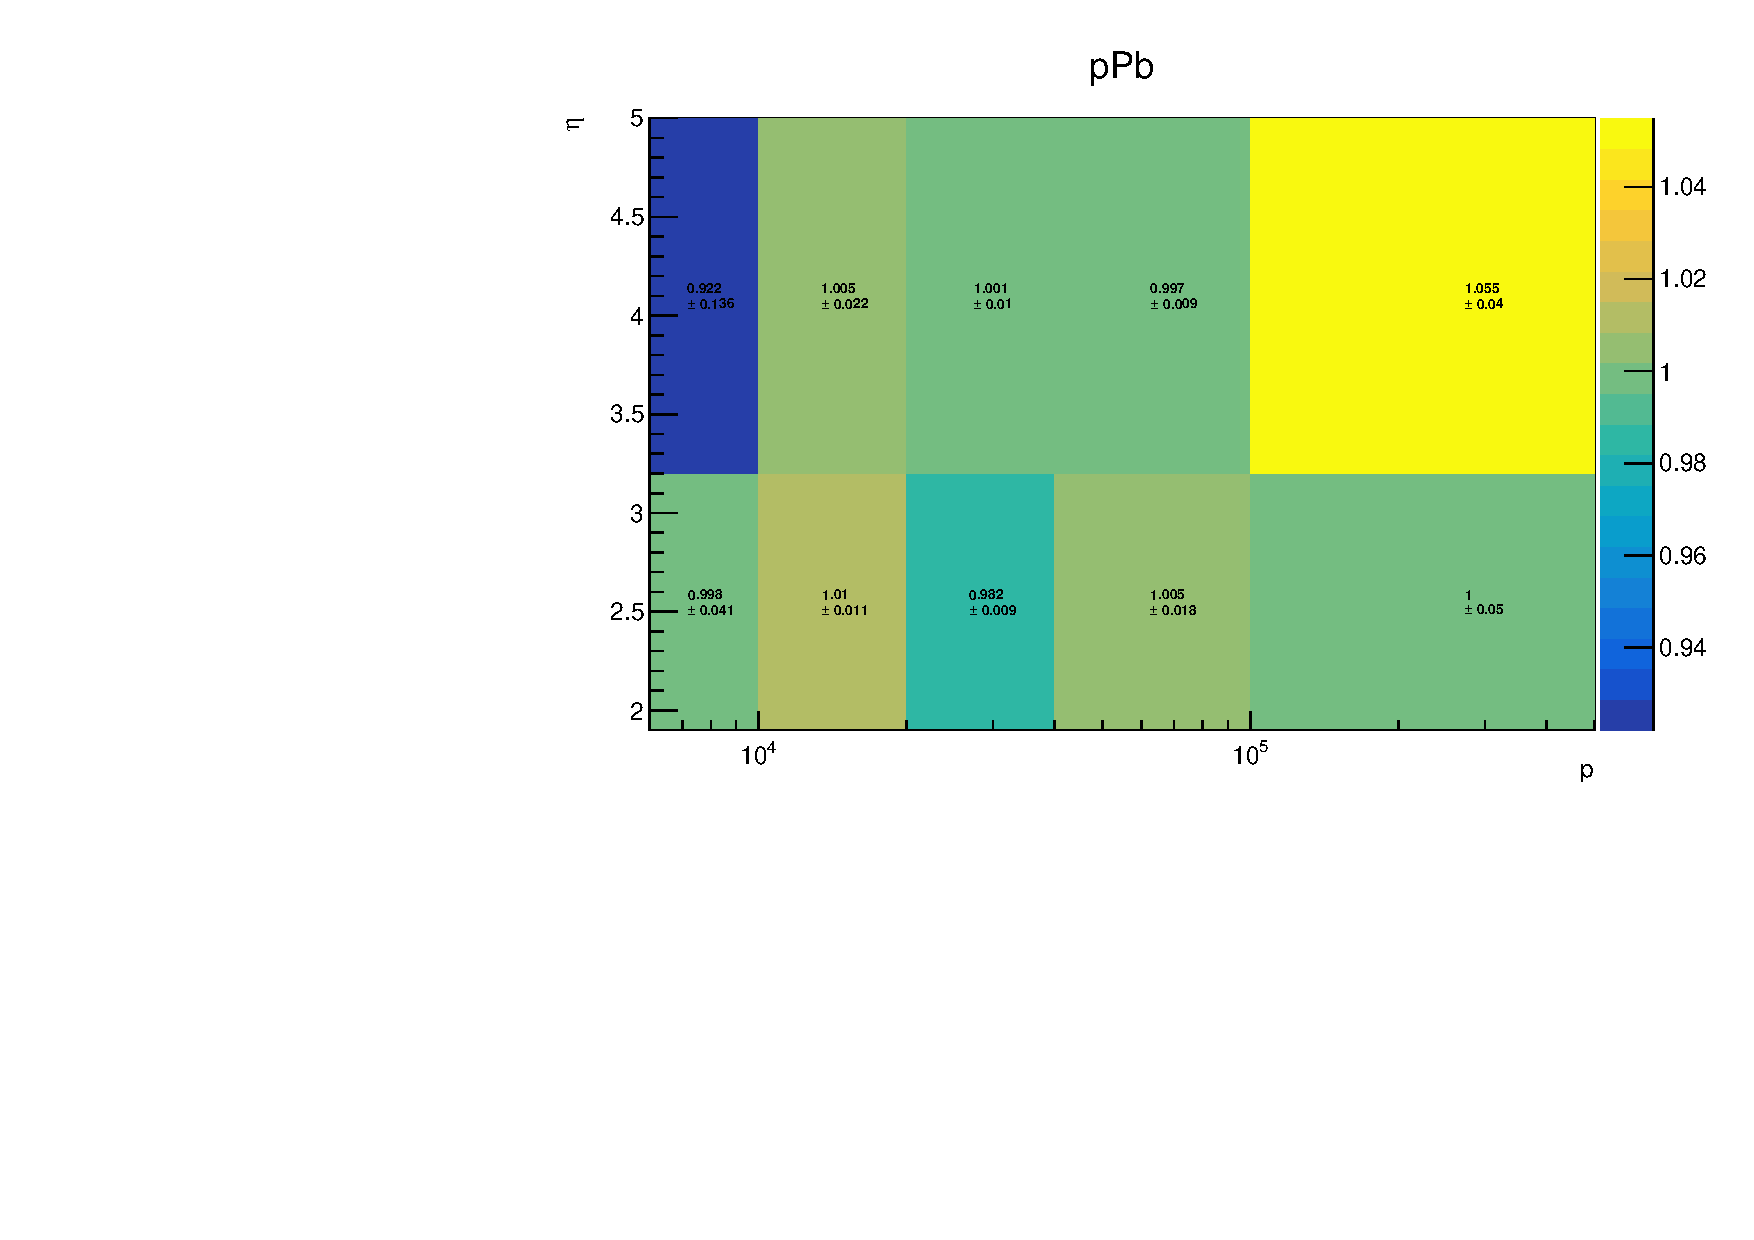
\includegraphics[width=0.49\linewidth]{pdf/pPb/Workdir/TrackCalib/pPb.pdf}
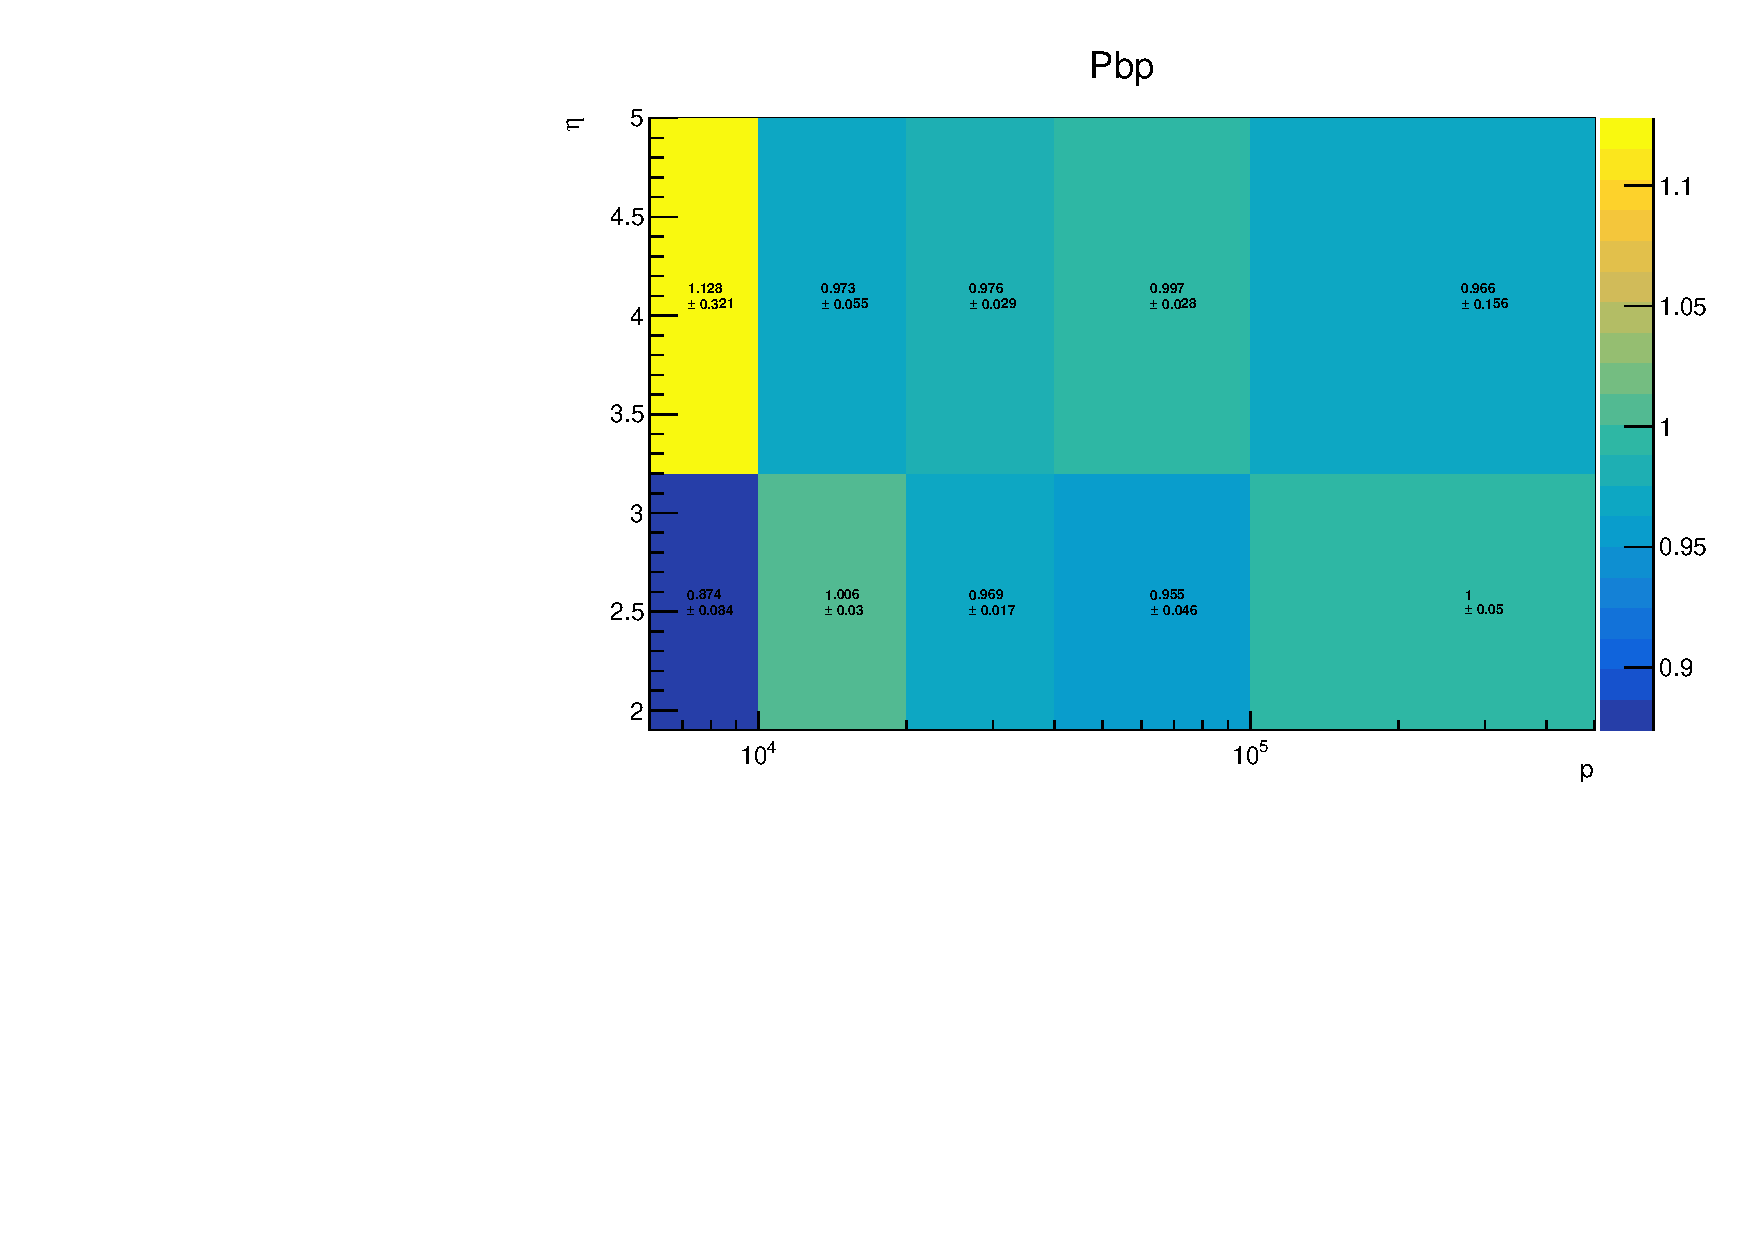
\includegraphics[width=0.49\linewidth]{pdf/pPb/Workdir/TrackCalib/Pbp.pdf}
\end{center}
	\caption{Ratio between data and $p$Pb (left) and Pb$p$ simulation of per-track tracking efficiency in bins of the track $\eta$ and $p$.
    }
\label{TrackTable}
\end{figure}

From Eq.~\ref{EffRatio} we can see that, we calculate the ratio of all the efficiencies $R_{eff}$ (except for acceptance efficiencies) as a whole part, since they are all calculated with full-simulation Monte Carlo sample. Another reason is, when calculating \effReco, \effID and \effTrigger, 500 random tables of \pt and $y^*$ from high- and low-multiplicity samples are generated (1000 in total) for both \jpsi and \psitwos in $p$Pb and Pb$p$ configurations and introduced to correct the imperfection on simulation to data. For a certain trial, the re-weight on \pt (or $y^*$) may under- or over-estimate  \effReco, \effID and \effTrigger simultaneously, it is hard to determine the dependence between these efficiencies. So a good way is to calculate them as a whole, each time a certain random re-weight table is introduced. The definition of $R_{eff}$ is in Eq.~\ref{Reff}.
\begin{equation}
R_{eff}\bigg|_{Mult. \ bin} = 
\frac{\ensuremath{\epsilon_{\mathrm{Reco\&Sel,\jpsi}}}\cdot\ensuremath{\epsilon_{\mathrm{MuonID,\jpsi}}}\cdot\ensuremath{\epsilon_{\mathrm{Trigger,\jpsi}}}}{\ensuremath{\epsilon_{\mathrm{Reco\&Sel,\psitwos}}}\cdot\ensuremath{\epsilon_{\mathrm{MuonID,\psitwos}}}\cdot\ensuremath{\epsilon_{\mathrm{Trigger,\psitwos}}}}\bigg|_{Mult. \ bin}.
\label{Reff}
\end{equation}
Similarly, 1000 random tables for data-over-simulation single tracking efficiency ratio are generated and introduced into the 1000 trials, and 1000 random tables for efficiency table obtained from PIDCalib package are introduced in each trial as well to calculate PID efficiencies, and hence, $R_{eff}$, as stated in the following part. So we will give an overall estimation (values and uncertainties) for $R_{eff}$ after introduced \effID and \effTrigger.

\subsection{PID efficiency}
The PID efficiency is defined as 
\begin{equation}
    \effID(\pt,y^*)=\frac{\jpsi(\psitwos) \mathrm{ \ satisfying \ PID \ selection \ in \ bin \ }(\pt,y^*)}{\jpsi(\psitwos)\mathbf{ \ selected \ in \ bin \ }(\pt,y^*)}.
\end{equation}
The PID efficiency for muons is taken from data using calibration tables (PIDCalib tables) obtained from control samples, namely \jpsi candidates. These calibration tables give the efficiency of the PID selections as a function of the pseudo-rapidity, of the total momentum of the muon tracks and of the track multiplicity of the event estimated from the number of hits in the SPD. They are available for the $pp$, $p$Pb and Pb$p$ data taking. 
The muon ID efficiency in each $(\pt,y^*)$ bin is then calculated by averaging the muon ID efficiency of each candidate in the bin, which is the product of the muon ID efficiencies of the two muons from the efficiency table, according to their $(p, \eta, nSPDhits)$ values. As mentioned above, calculation on \effID for \jpsi and \psitwos is only a section of calculation of $R_{eff}$. So 1000 random tables are generated from the PIDCalib efficiency table and introduced to each trial of $R_{eff}$ calculations.

\subsection{Trigger efficiency}
The trigger efficiency is defined as follows
\begin{equation}
    \effTrigger(\pt,y^*)=\frac{\jpsi(\psitwos)\mathrm{ \ TOS of \ L0 \ and \ HLT1 \ in \ bin \ }(\pt,y^*)}{\jpsi(\psitwos)\mathbf{ \ selected \ in \ bin \ }(\pt,y^*)},
\end{equation}
where the selection includes here the PID requirements. The efficiencies are computed with the simulated samples, applying on them the simulation of the PID. Note that since the analysis is done on the TURBO candidates, the efficiency of the HLT2 is included in the reconstruction, PID and selection efficiencies. When calculating the trigger efficiencies for \jpsi and \psitwos, same random tables generated from re-weight tables of \pt and $y^*$ are used as that used in \effReco and \effID above for each one of the 1000 trials.

\subsection{Total efficiency}
Finally, the 1000 ratios of all the efficiencies except geometric acceptance $R_{eff}$'s are fitted with a Gaussian function. Hence, we can calculate the ratio of total efficiencies $R_{tot}=R_{acc}\times R_{eff}$ with systematic uncertainties arised from,
\begin{itemize}
    \item re-weight of \pt distribution from high- and low-multiplicity samples,
    \item re-weight of $y^*$ distribution from high- and low-multiplicity samples,
    \item uncertainties due to the limit calibration sample size in PIDCalib efficiency table,
    \item uncertainties of data-over-simulation ratio of per tracking efficiency.
\end{itemize}
Systematic uncertainties from other sources will be discussed in Sec~\ref{Systematic uncertainty}. As an example, the fit results for $R_{eff}$ in different $N_{\rm tracks}^{\rm PV}$ classes for $p$Pb configuration are shown in Figure~\ref{ReffPlots}. The corresponding values of $R_{eff}$ with uncertainties mentioned above are summarized in Table~\ref{ReffTable_PVNTRACKS_pPb}. Fit plots and summary tables for other multiplicity variables and configurations can be found in appendix.
\begin{figure}[!tpb]
\begin{center}
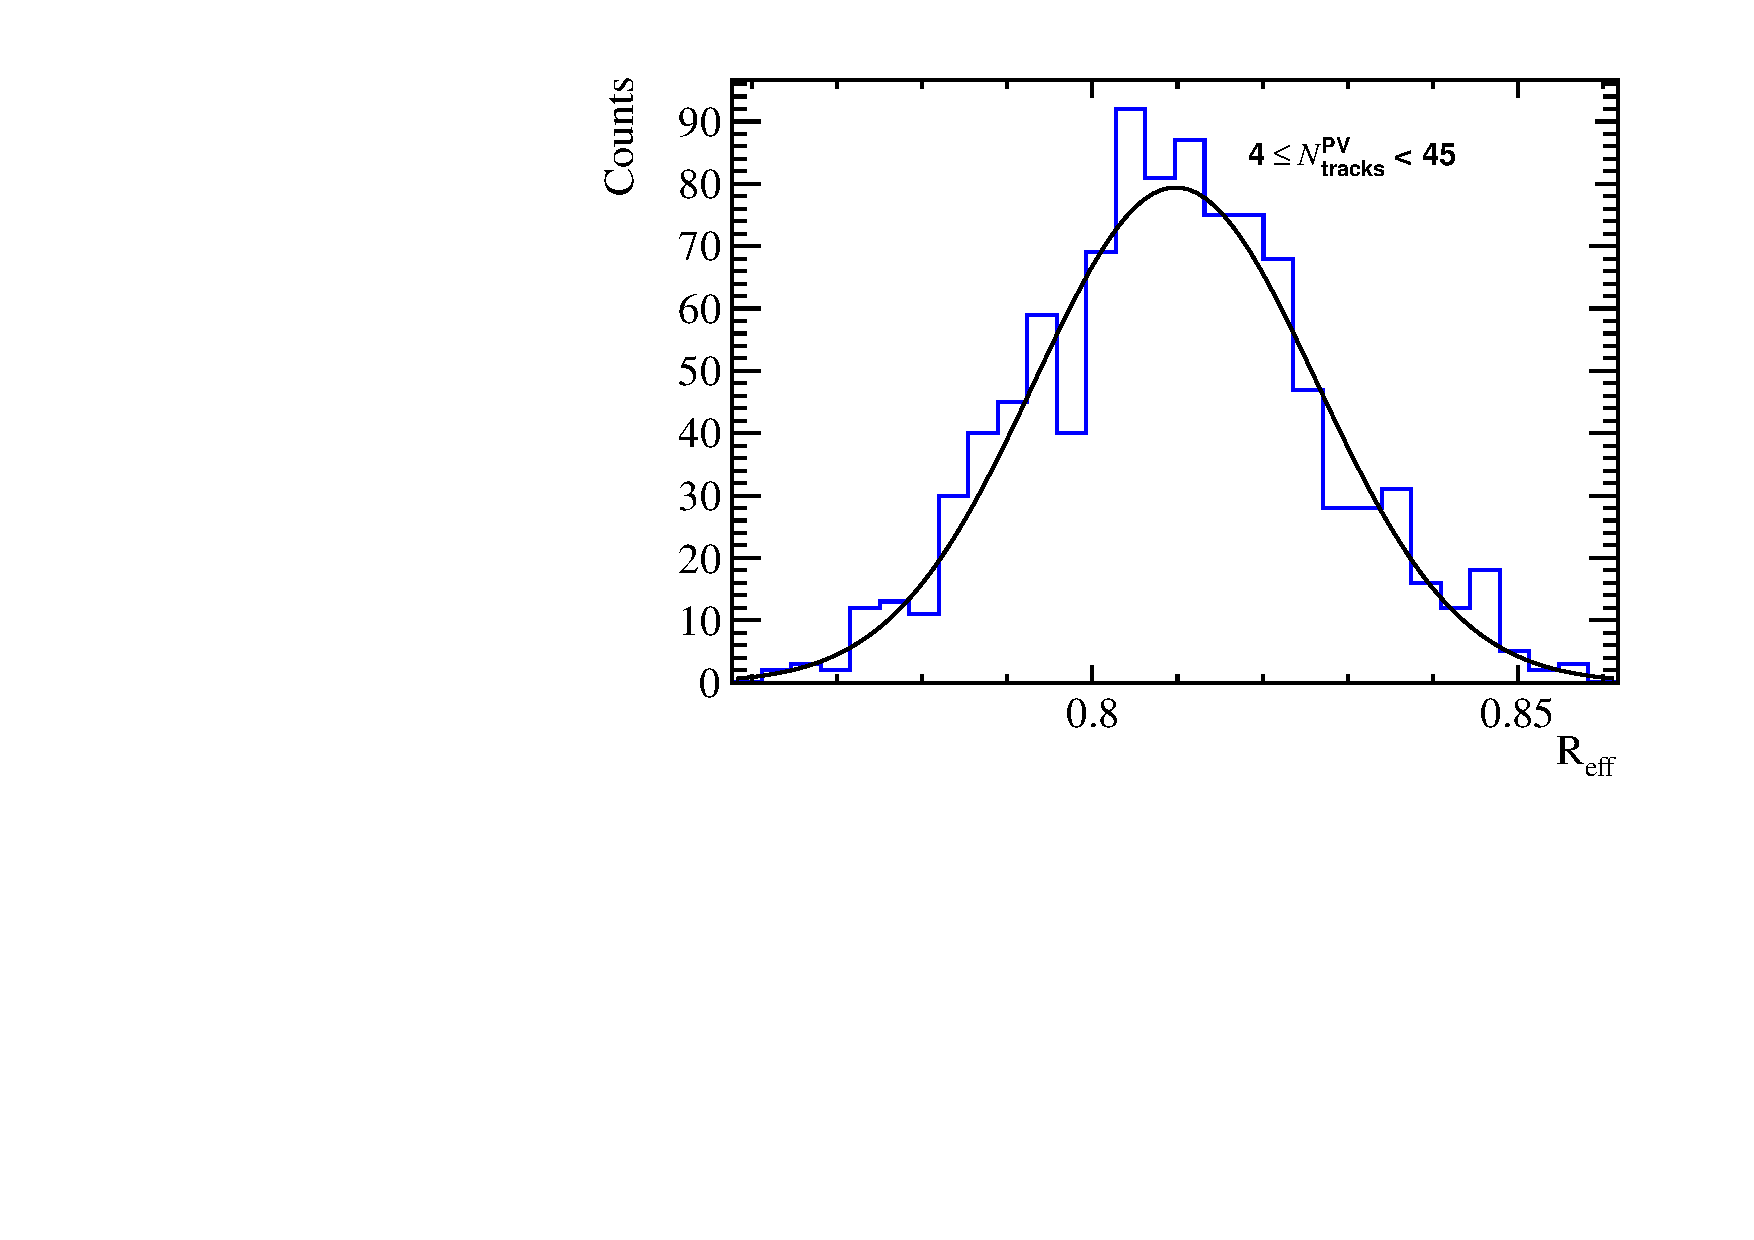
\includegraphics[width=0.49\linewidth]{pdf/pPb/Workdir/Eff_RecselPIDTrigger/n1.pdf}
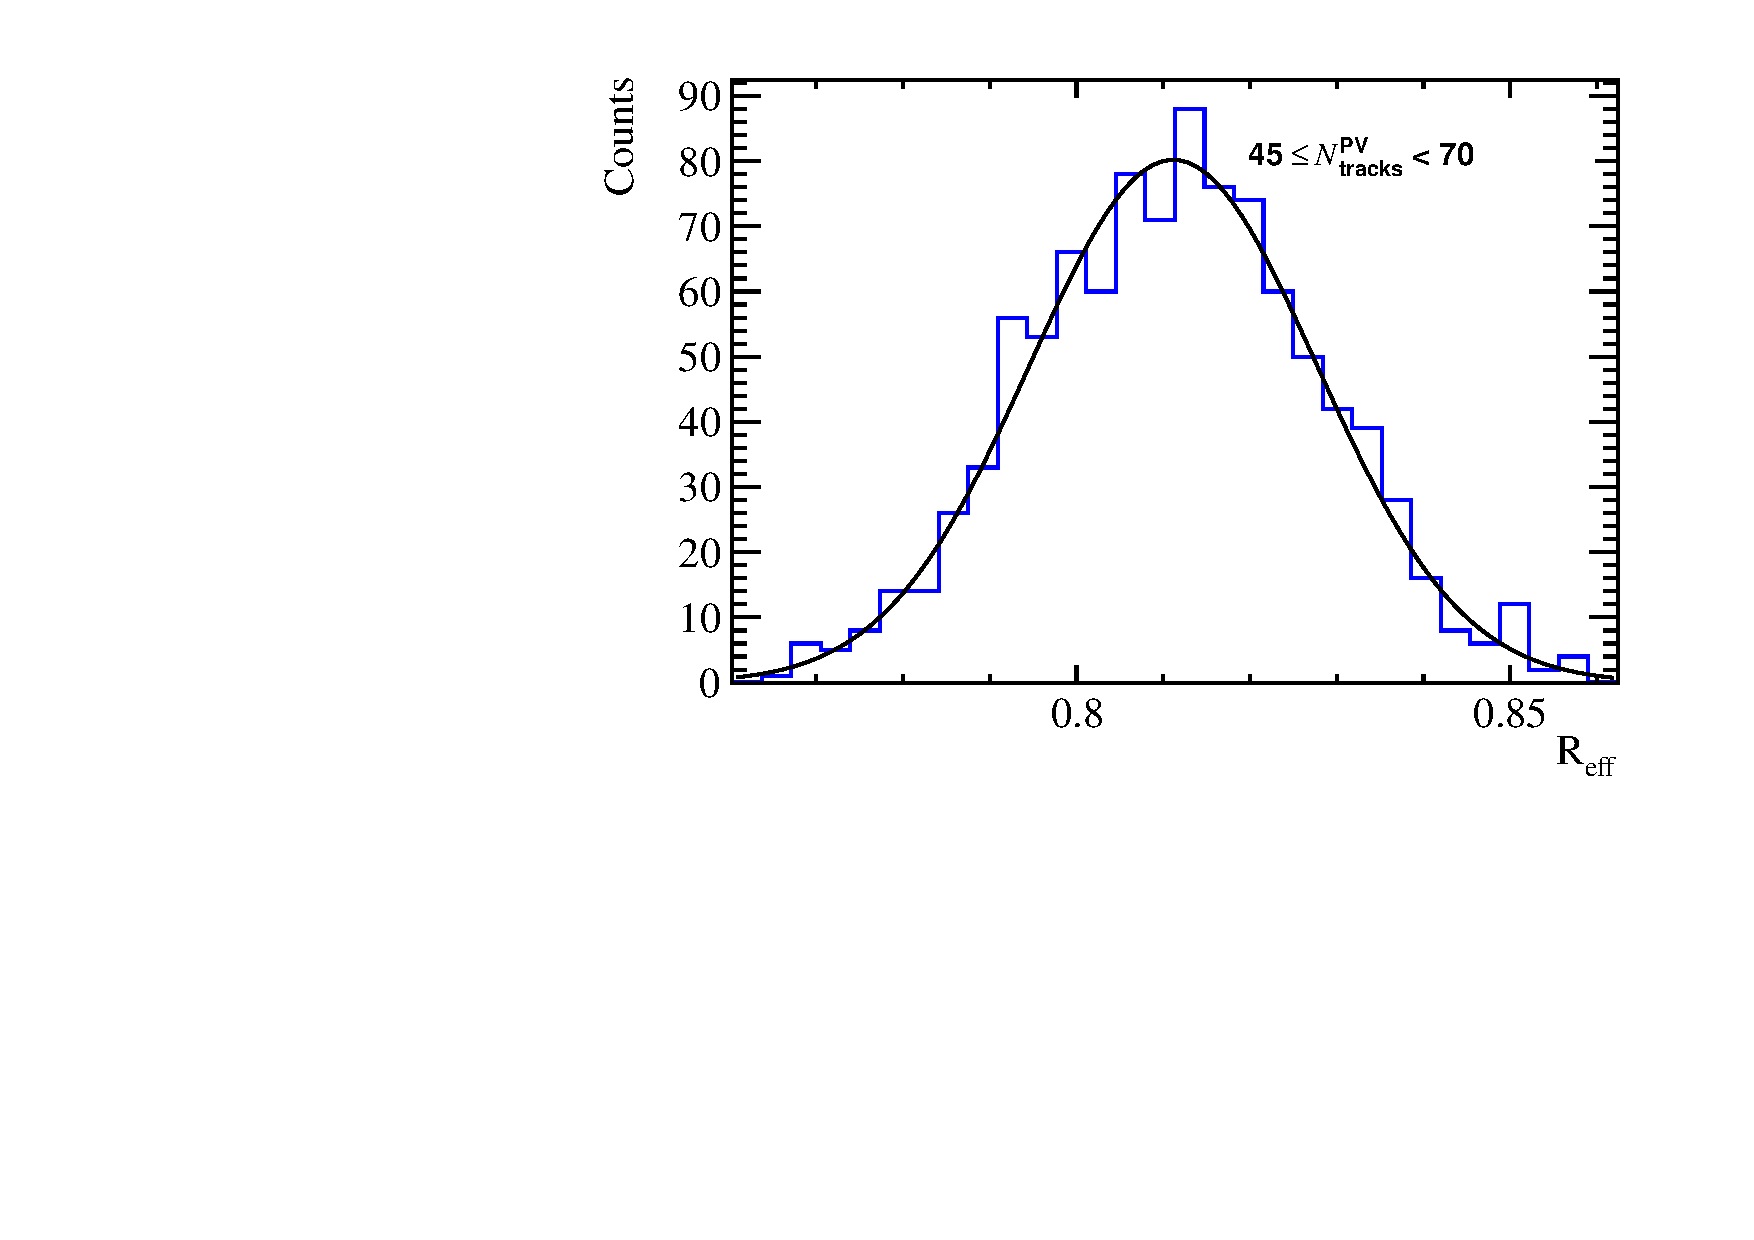
\includegraphics[width=0.49\linewidth]{pdf/pPb/Workdir/Eff_RecselPIDTrigger/n2.pdf}
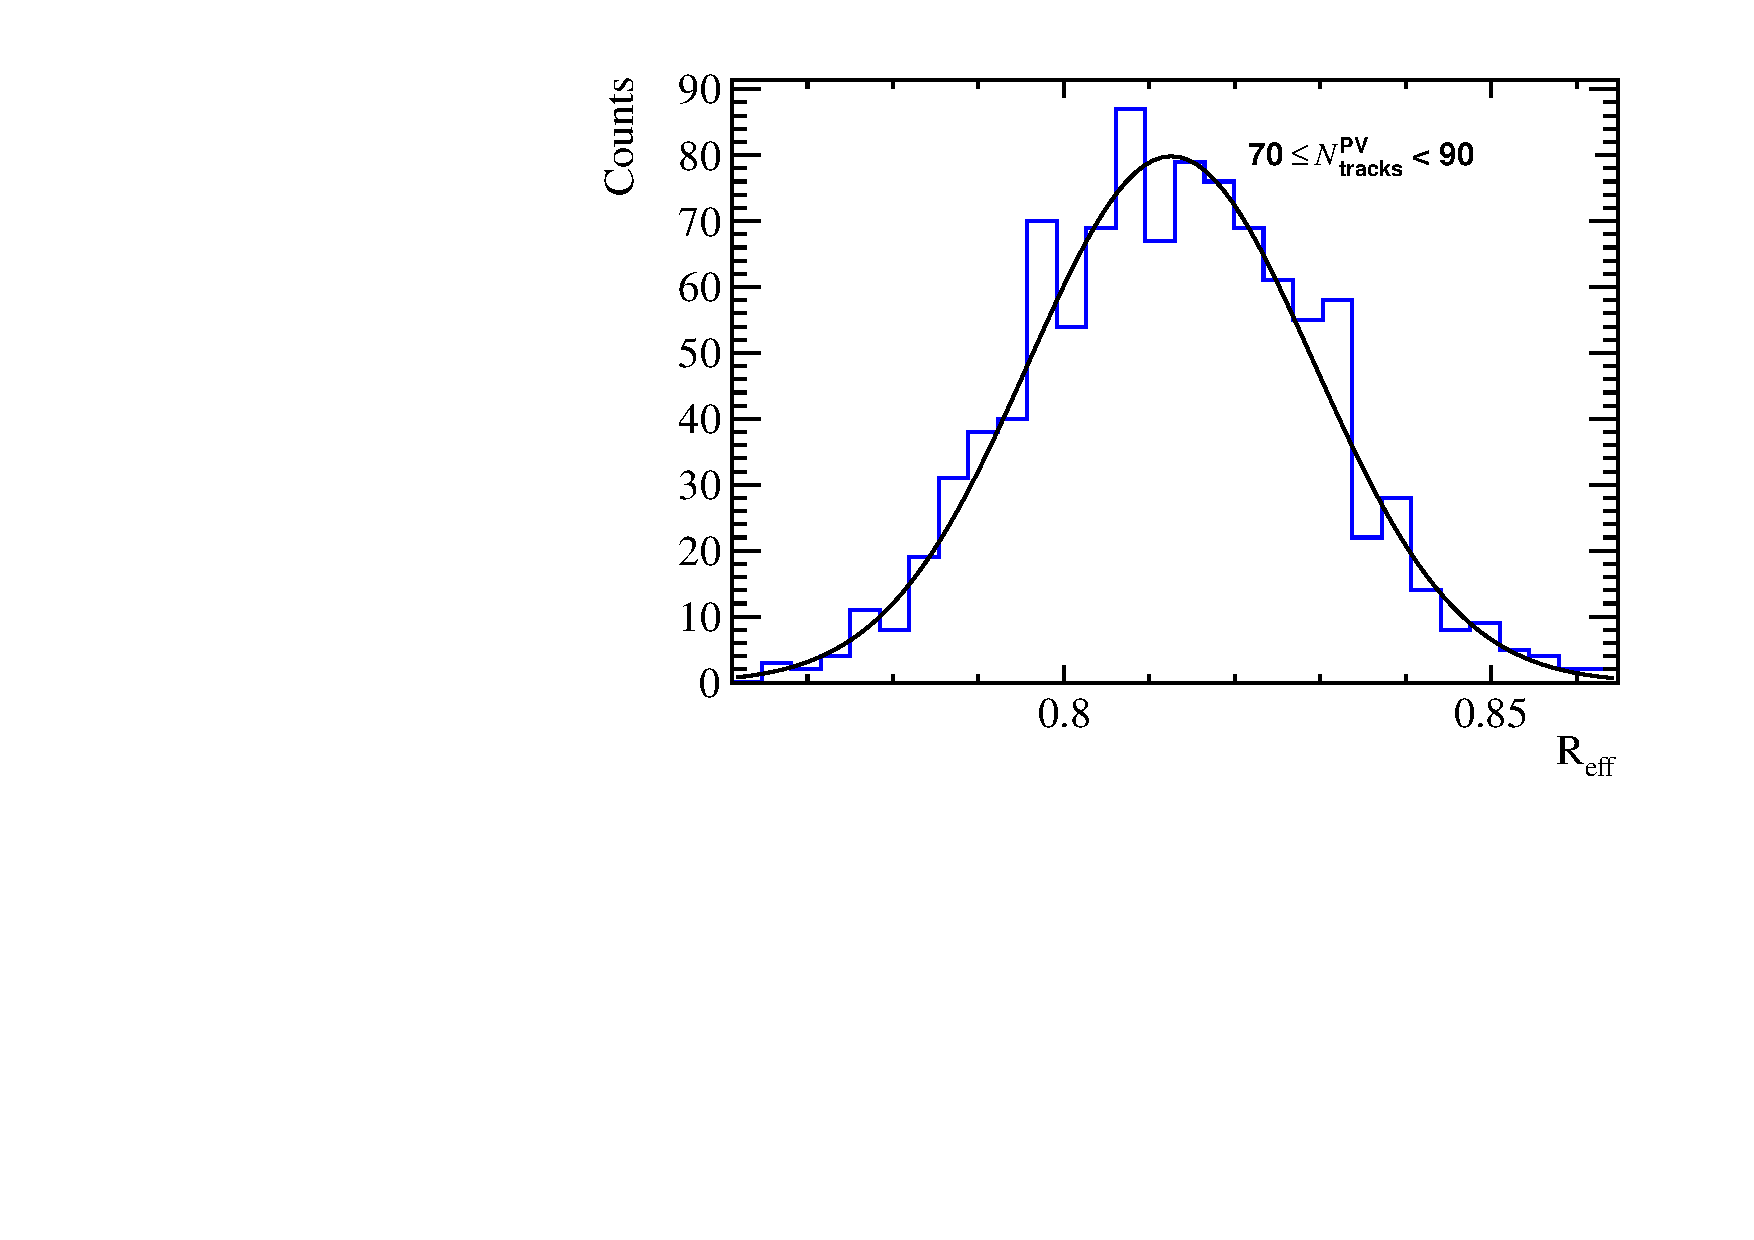
\includegraphics[width=0.49\linewidth]{pdf/pPb/Workdir/Eff_RecselPIDTrigger/n3.pdf}
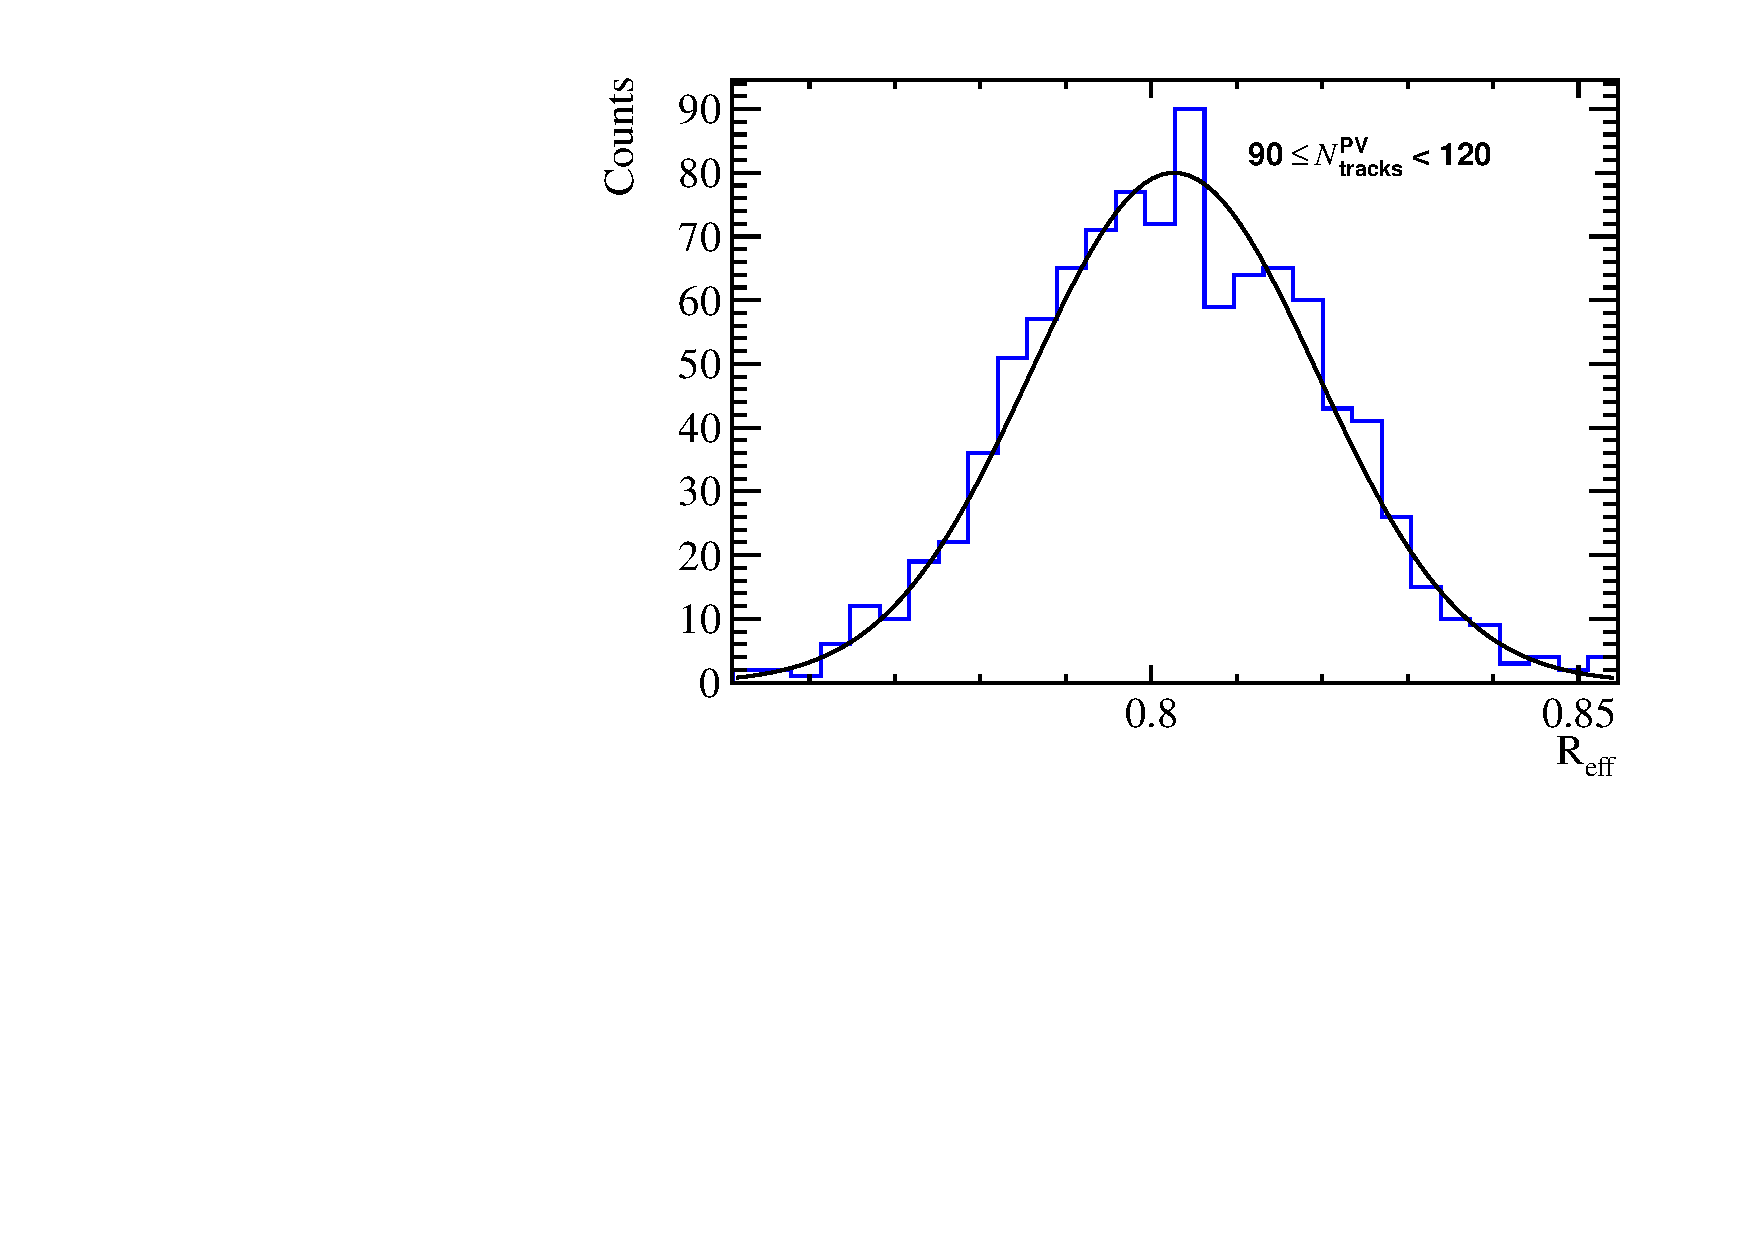
\includegraphics[width=0.49\linewidth]{pdf/pPb/Workdir/Eff_RecselPIDTrigger/n4.pdf}
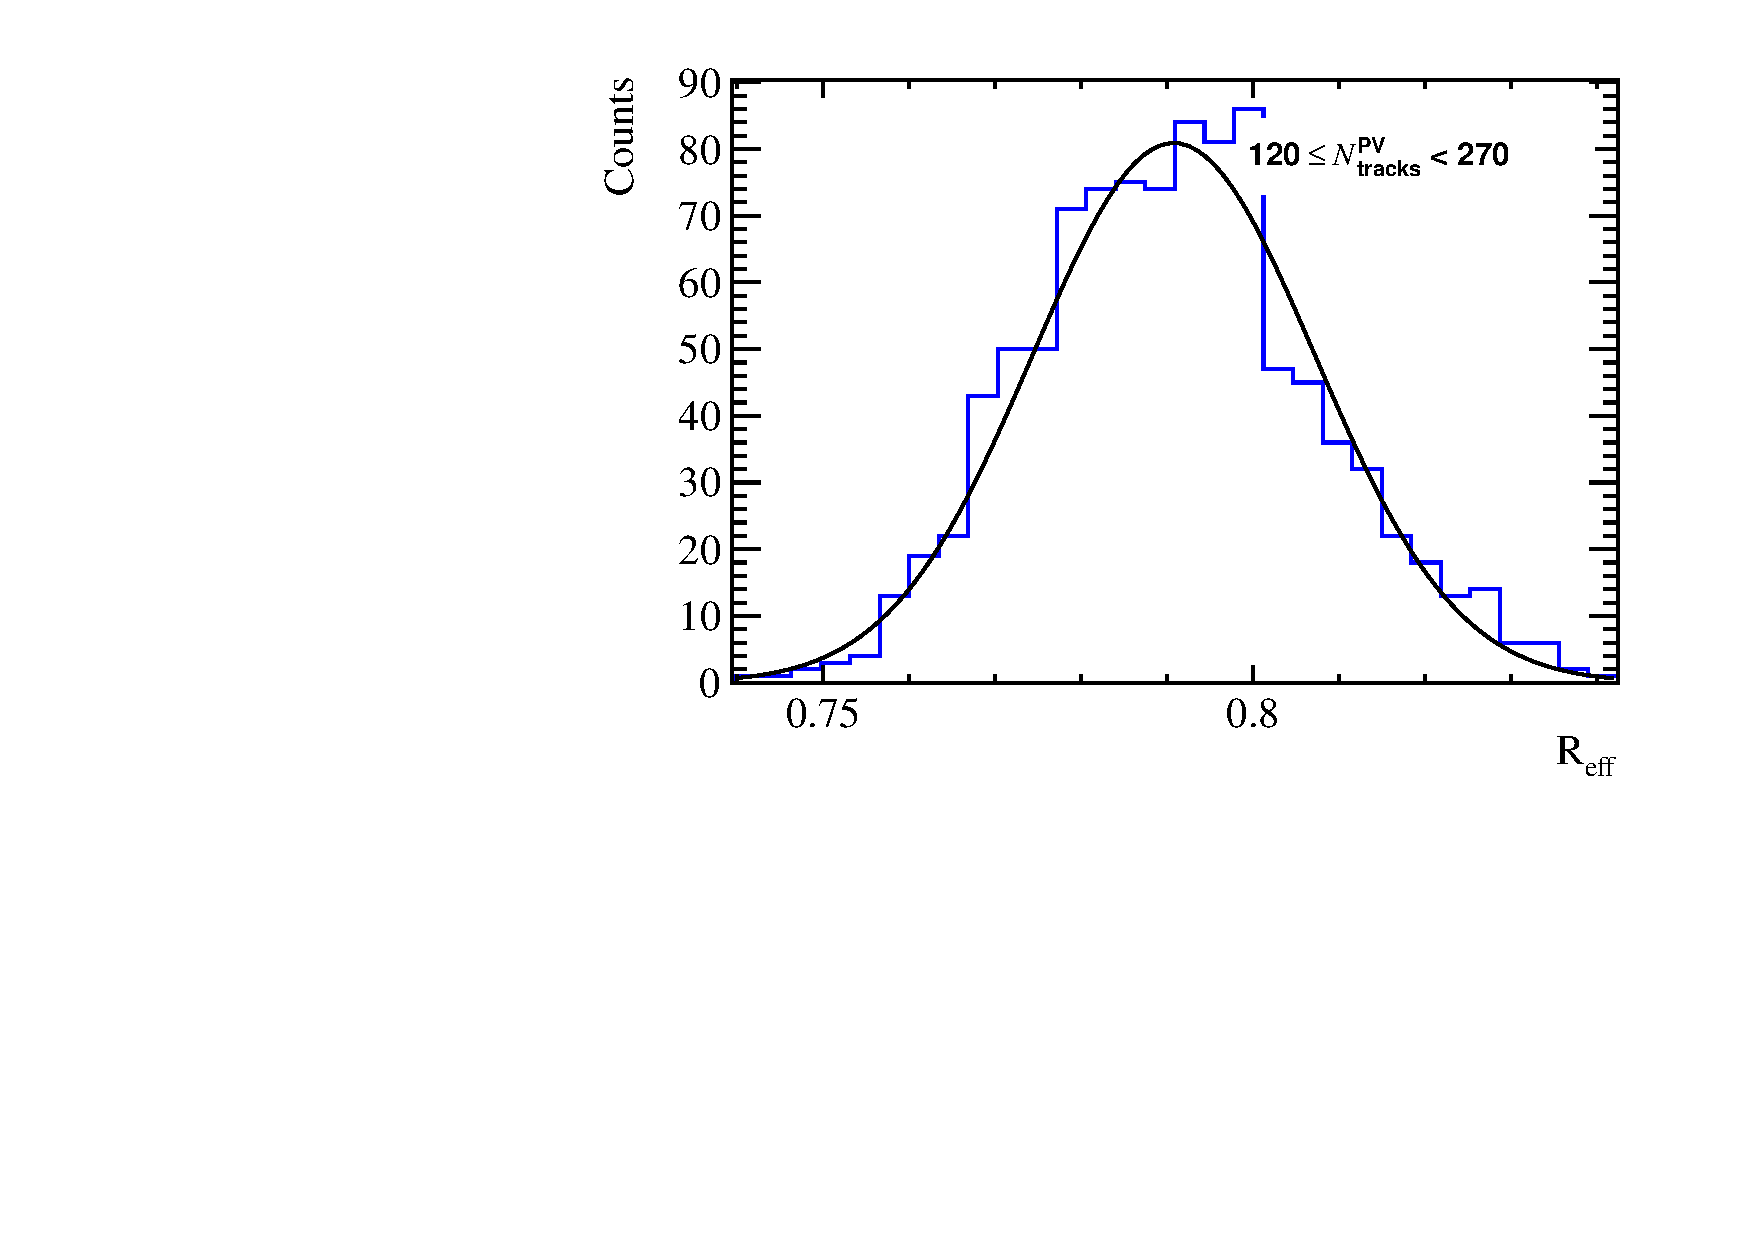
\includegraphics[width=0.49\linewidth]{pdf/pPb/Workdir/Eff_RecselPIDTrigger/n5.pdf}
\end{center}
\caption{
	Fit Gaussian functions on the distributions of 1000-trial $R_{eff}$'s in different $N_{\rm tracks}^{\rm PV}$ classes.}
\label{ReffPlots}
\end{figure}
\begin{table}[H]
\centering
\caption{$R_{eff}$ in different $N_{\rm tracks}^{\rm PV}$ regions in $p$Pb configuration.}
\begin{center}
\begin{tabular}{c|c}
\hline
$4 \leq \mathrm{N_{\rm tracks}^{\rm PV}} < 45$ & $0.810 \pm 0.021$ \\
\hline
$45 \leq \mathrm{N_{\rm tracks}^{\rm PV}} < 70$ & $0.811 \pm 0.020$ \\
\hline
$70 \leq \mathrm{N_{\rm tracks}^{\rm PV}} < 90$ & $0.813 \pm 0.021$ \\
\hline
$90 \leq \mathrm{N_{\rm tracks}^{\rm PV}} < 120$ & $0.803 \pm 0.021$ \\
\hline
$120 \leq \mathrm{N_{\rm tracks}^{\rm PV}} < 270$ & $0.791 \pm 0.021$ \\
\hline
\end{tabular}
\end{center}
\label{ReffTable_PVN_pPb}
\end{table}

